\chapter{Publications}
\label{chap:publications}

This chapter presents the three published works that form the scholarly core of the PhD, arranged chronologically (starting with earliest) to reflect the progression of the research. It builds on earlier chapters, which established the thesis aims, objectives, and the development of the Thonny-py5mode software. Together, these publications mark key milestones in the research journey, spanning the design of Python-based curricula, the exploration and development of new tools, and the empirical evaluation of Thonny-py5mode through a user study. The list below situates each publication within the broader stages of the PhD:

\begin{enumerate}

\item \textbf{Publication \ref{sec:no-starch} $-$ Stage: Processing.py and curriculum foundations.}  
This phase focused on establishing a curriculum for teaching Python through visual learning contexts, culminating in the sole-authored book \textit{\nameref{sec:no-starch}}. This book captures and formalises the educational approaches that initially framed the research.

\item \textbf{Publication \ref{sec:mtap} $-$ Stage: Transition to new tools and the development of Thonny-py5mode.}  
The discontinuation of Processing.py created a gap for a new Python-based creative coding environment. This led to the development of Thonny-py5mode: a plugin intended to replace and extend Processing's Python Mode. The \textit{\nameref{sec:mtap}} article positions Thonny-py5mode within the broader context of Python creative coding tools, highlighting its contribution to programming education.

\item \textbf{Publication \ref{sec:jise} $-$ Stage: Empirical testing and evaluation.}  
This component of the research involved an empirical evaluation of Thonny-py5mode in a 100-level university Python course. The \textit{\nameref{sec:jise}} article reports on this study, assesses the plugin's effectiveness through the lens of Task--Technology Fit, and discusses its broader implications for related educational contexts.

\end{enumerate}

The \nameref{chap:presentation-outputs} chapter documents the talks, workshops, and demonstrations that underpinned the publications presented here. Figure~\ref{fig:publications-chart} maps the three publications onto the PhD timeline---using their submission rather than publication dates---thereby illustrating the formative role of presentation outputs in their development.

\begin{figure}[htbp]
\centering
\medskip
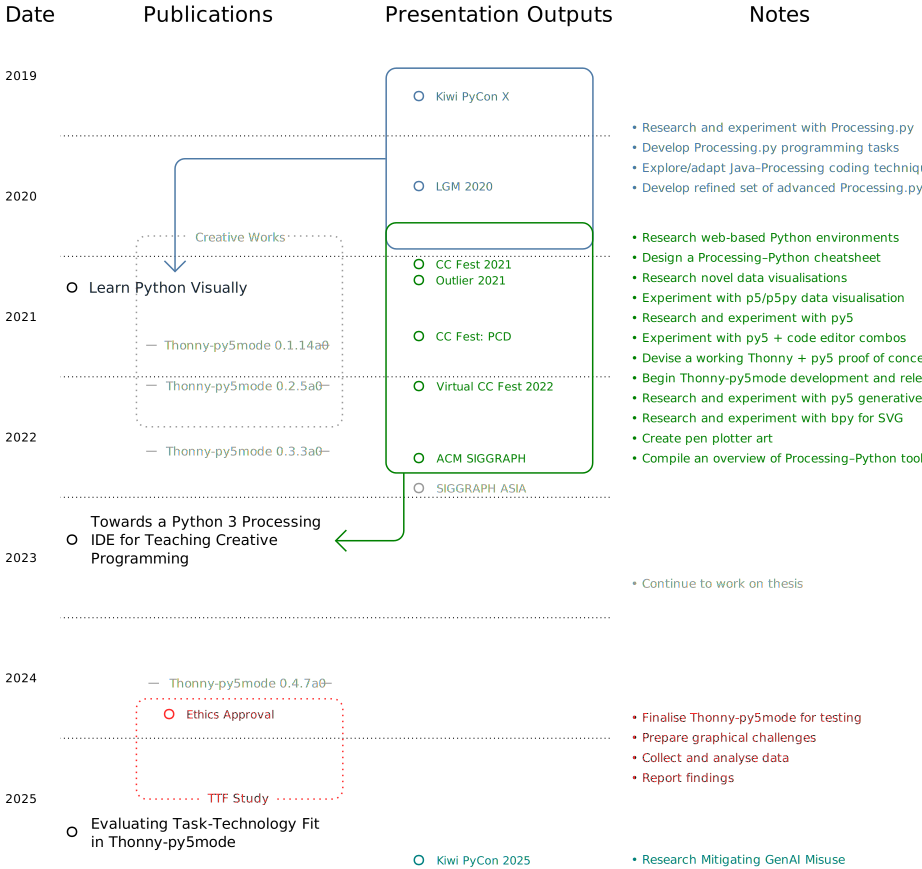
\includegraphics[width=1.0\textwidth]{chapters/chapter04-publications/publications-chart}
\smallskip
\caption{Timeline of publications, highlighting the integration of presentation outputs (talks, workshops, and demonstrations) into the research process. Diagram by the author.}
\label{fig:publications-chart}
\end{figure}

The \textit{Publications} column lists the three works discussed in this chapter, shown in \textbf{bold black type}. Within this column, several \textcolor{gray}{\textit{--- Thonny-py5mode...}} entries indicate individual Thonny-py5mode releases. Dotted-outline cells mark the periods of producing the \textit{Creative Works} (covered in the \nameref{chap:creative-works} chapter) and conducting the empirical evaluation of Thonny-py5mode (\textit{TTF Study}). The \textit{Notes} column summarises the processes and steps that defined each stage.

Viewed within the context of this PhD by folio/publication, the sole-authored book and two peer reviewed Q1/Q2 journal articles balance practical impact with scholarly rigour. \textit{\nameref{sec:no-starch}} serves as a resource for educators integrating Python-based creative coding into curricula, while the journal articles contribute to academic discussion surrounding Python tools for visual learning contexts. Collectively, these publications address four research objectives outlined in the ``\nameref*{chap:introduction}'' chapter: \hyperref[ro:tool-development]{Tool Development}, \hyperref[ro:educational-materials]{Educational Materials}, \hyperref[ro:empirical-evaluation]{Empirical Evaluation}, and \hyperref[ro:broader-dissemination]{Broader Dissemination}.

As outlined in Figure~\ref{fig:literature-review-conceptual-map} in the ``\nameref*{chap:literature-review}'' chapter, the journal articles engage with much of the relevant literature, as do the \nameref{chap:presentation-outputs} and, to a lesser extent, the \nameref{chap:creative-works}. Given the folio/publication thesis format, some of the literature in the journal articles unavoidably overlaps with the \nameref*{chap:literature-review}. Specifically---

\begin{itemize}

\item While the ``\nameref*{chap:literature-review}'' chapter also covers prominent creative coding environments, the article \textit{\nameref{sec:mtap}} extends this analysis to explore Python-3-specific creative coding environments in greater depth.

\item The other article, \textit{\nameref{sec:jise}}, reiterates some of the general and introductory literature on creative coding environments in a more condensed form. However, it also provides an additional review of scholarship supporting the Task--Technology Fit framework, which is central to its study.

\end{itemize}

The next section (\ref{sec:no-starch}) reviews the content and development of the book \textit{\nameref{sec:no-starch}}, which cannot be reproduced in full here because of its length and copyright restrictions. Following that, the subsequent sections (\ref{sec:mtap}, \ref{sec:jise}) present the two journal articles in their preprint (submitted) form, which do not incorporate revisions made after peer review. Publishers permit the distribution and archiving of these versions, which exclude publisher formatting and instead follow the style and conventions of the thesis.

%%%%%%%%%%%%%%%%%%%%%%%%%%%%%%%%%%%%%%%%%%%%%%%%%%%%%%%%%%%%%%%%%%%%%%%%%%%%%%%
%%%%%%%%%%%%%%%%%%%%%%%%%%%%%%%%%%%%%%%%%%%%%%%%%%%%%%%%%%%%%%%%%%%%%%%%%%%%%%%

\cleardoublepage
\section{Learn Python Visually: Creative Coding with Processing.py}
\label{sec:no-starch}
\vspace{1.5em}
\begin{outputmeta}
\textbf{Publisher}: No Starch Press \\
\textbf{Publisher URL}: \url{https://nostarch.com} \\
\textbf{Author(s)}: Bunn, T. \\
\textbf{Date published}: 20 July 2021 \\
\textbf{ISBN-13}: 978-1-7185-0096-9 \\
\textbf{Print length}:‎ 296 pages \\
\textbf{Catalogue entry}: \url{https://nostarch.com/Learn-Python-Visually} \\
\textbf{Publication evidence}: See Appendix \ref{appendix:no-starch-cover}
\end{outputmeta}
\subsection{Background \& Context}

\textit{Learn Python Visually} (Figure~\ref{fig:book-cover-photo}) represented a significant component of this PhD research, concluding the initial phase of investigation into- and development of novel Python-based creative coding techniques. Aimed at beginner coders and readers transitioning from other programming backgrounds, the book employs Processing's Python Mode (Processing.py) as its pedagogical foundation, combining Python's accessibility with Processing's multimedia capabilities.

\begin{figure}[htbp]
\centering
\includegraphics[width=1\textwidth]{chapters/chapter04-publications/no-starch/book-cover-photo}
\caption{\textit{Learn Python Visually: Creative Coding with Processing.py}. Photo by the author.}
\label{fig:book-cover-photo}
\end{figure}

The book's strength and novelty lie in its visual and practical take on Python instruction. Each chapter builds progressively upon the last, moving from fundamental concepts toward more sophisticated creative coding techniques. This approach directly aligns with the overarching aim of the thesis: enhancing Python programming education through creative computing environments, and specifically the \hyperref[ro:educational-materials]{Educational Materials} and \hyperref[ro:broader-dissemination]{Broader Dissemination} objectives. Two presentations in particular, \nameref{sec:processing.py-creative-coding-with-python} and \nameref{sec:processing-python-mode-for-creative-coding-and-teaching}, provide further insight into the activities and research that informed the book's development. 

No Starch Press is a respected independent publisher specialising in technical and educational titles. Established in 1994, it has built a strong reputation for publishing accessible yet rigorous works on programming, cybersecurity, and STEM education, including bestsellers such as \textit{Python Crash Course}, \textit{Python for Kids}, \textit{How Linux Works}, and \textit{Hacking: The Art of Exploitation}. Its titles---widely adopted by learners, educators, and professionals---have received industry recognition, including Independent Publisher Book Awards (from \textit{Independent Publisher} magazine) and inclusion in the prestigious \textit{Communication Arts Design Annual}. This status underscores the book's credibility as both a practical learning resource and a contribution to Python-based programming education~\cite{no_starch_press_about_2025}.

Paddy Gaunt, who served as the book's technical reviewer, studied engineering at Cambridge University (UK). Since 2012, he has maintained pi3d: a Python library designed to deliver high-speed 3D graphics on Raspberry Pi microcomputers~\cite{bunn_learn_2021}.

\textit{Learn Python Visually} is available worldwide in both print and digital formats. It has received favourable reviews on Amazon.com\footnote{~\url{https://www.amazon.com/Learn-Python-Visually-Tristan-Bunn/dp/1718500963}} where it features editorial endorsements from Saber Khan (Education Community Director of the Processing Foundation), Dr.~Ralf Biedert (Principal Engineer at Tobii AB), and Alfred Abusomwan (Techs Blog). As of June 2025, the book had achieved 2,622 direct sales (Appendix \ref{appendix:no-starch-royalty-statement}). It was also included in two Humble Bundle collections: \textit{Machine Learning by No Starch Press} (August 2021) and \textit{Python by No Starch Press} (May 2023), that sold 17,669 and 10,881 bundles, respectively~\cite{humble_bundle_inc_machine_2021, humble_bundle_inc_humble_2023}. 

In addition to direct and bundled sales, the book is distributed internationally through No Starch Press partners, including digital platforms such as O'Reilly Online Learning\footnote{~\url{https://www.oreilly.com/library/view/learn-python-visually/9781098128937}} and through academic library collections, further extending its educational reach. Penguin Random House distributes No Starch Press printed titles in the USA and worldwide~\cite{no_starch_press_sales_2025}.

\textit{Learn Python Visually} integrates visual learning throughout its chapters, requiring learners to program output that expresses computational methods through graphical outputs, animations, data visualisations, 2D simulations, and interactive interfaces. In this way, it places emphasis on immediate, observable results to elucidate abstract concepts and support intuitive understanding. The book is printed in full colour, incorporating visual explanations in addition to the results of different code samples. Figures~\ref{fig:book-p190-p205} and~\ref{fig:book-p210-p225} present a sample selection of 16 pages each.

\begin{figure}[htbp]
\centering
\includegraphics[width=\textwidth]{chapters/chapter04-publications/no-starch/book-p190-p205}
\caption{Excerpt from the author's book \textit{Learn Python Visually} (pp.~190--205), published by No Starch Press. This section introduces trigonometric functions and waveforms, and demonstrates the generation of Lissajous figures using Python. Source:~\cite{bunn_learn_2021}.}
\label{fig:book-p190-p205}
\end{figure}

\begin{figure}[htbp]
\centering
\includegraphics[width=\textwidth]{chapters/chapter04-publications/no-starch/book-p210-p225}
\caption{Excerpt from the author's book \textit{Learn Python Visually} (pp.~210--225), published by No Starch Press. This section introduces object-oriented principles through the generation of an amoeba simulation using Python. Source:~\cite{bunn_learn_2021}.}
\label{fig:book-p210-p225}
\end{figure}

The early chapters cover introductory concepts, such as installation procedures, basic syntax, arithmetic operations, and the principles of drawing with code. Once readers are familiar with the fundamentals, later chapters build on these foundations, shifting focus to concepts that require more programmatic reasoning---control flow, iteration, randomness, motion, transformations, data visualisation, and constructing a user interface. The following outline provides a brief overview of each chapter's contents:

\begin{quote}

\noindent\textbf{Chapter 1: Hello, World!} \\
Covers installation and setup for Processing Python Mode (Processing.py) and introduces the basics of drawing with code. Also: how computers manage colour, how to store and reuse values using variables, and how to perform basic arithmetic operations in Python.

\vspace{0.5em}
\noindent\textbf{Chapter 2: Drawing More Complicated Shapes} \\
Building on drawing essentials, readers move on to organic (non-geometric) shapes---defining these with points (vertices) and curves, which can describe almost any 2D form in code.

\vspace{0.5em}
\noindent\textbf{Chapter 3: Introduction to Strings and Working with Text} \\
Introduces Python's string features for manipulating text. To visualise these concepts, readers explore Processing functions for drawing text to the display window in different styles, colours, and fonts.

\vspace{0.5em}
\noindent\textbf{Chapter 4: Conditional Statements} \\
Moving into control flow, demonstrating how to write programs that make decisions and execute different actions in response to different situations. Again, readers explore these concepts through graphical output.

\vspace{0.5em}
\noindent\textbf{Chapter 5: Iteration and Randomness} \\
Covers repeating operations in Python, either a specified number of times or until a condition is met. Readers combine these techniques with randomness to generate tiled patterns.

\vspace{0.5em}
\noindent\textbf{Chapter 6: Motion and Transformation} \\
Introduces the \texttt{draw()} function for animated output. Also covers saving frames as images, transforming groups of visual elements, and employing real-time values for screensavers and clock displays.

\vspace{0.5em}
\noindent\textbf{Chapter 7: Working with Lists and Reading Data} \\
Unlocks techniques for managing and manipulating collections of values, leading to practical data visualisation examples that read in external CSV data to generate charts dynamically.

\vspace{0.5em}
\noindent\textbf{Chapter 8: Dictionaries and JSON} \\
Explores richer data structures and visualisation with JSON data, developing readers' skills to work with more complex and novel data visualisations.

\vspace{0.5em}
\noindent\textbf{Chapter 9: Functions and Periodic Motion} \\
Shows how dividing programs into reusable functions improves modularity and readability, then combines these techniques with trigonometric operations to generate elliptical and wave-type motions.

\vspace{0.5em}
\noindent\textbf{Chapter 10: Object-Oriented Programming and PVector} \\
Demonstrates object-oriented principles to structure programs that model real-world phenomena, guiding readers through programming a visually engaging amoeba simulation that leverages vector-based motion.

\vspace{0.5em}
\noindent\textbf{Chapter 11: Mouse and Keyboard Interaction} \\
Concludes the book by adding interactivity to Processing sketches, focusing on mouse and keyboard input to build a paint app. This requires event functions and techniques for controlling Processing's draw-loop behaviour.

\end{quote}

An Afterword discusses where readers might head next, pointing them to the Processing community forum and useful materials, including tutorials on working with Images \& Pixels, P3D for 3D work, and the broader Processing ecosystem of libraries (written for Java Mode but typically portable to Python Mode). It encourages translating Java examples, highlights Daniel Shiffman's \textit{The Nature of Code} (with Python ports), and discusses Python's applications in games, the web, data, and AI. Additionally, there is some discussion on adjacent creative-coding environments, including p5.js, JRubyArt, openFrameworks, OPENRNDR, and hardware programming with Arduino.

Notably, readers' prior experience in related areas, including other programming languages, will likely influence their comprehension and the pace at which they progress through the book. However, the text encourages detours wherever inspiration strikes and includes challenges and practical tasks at key moments to reinforce conceptual understanding and promote active learning. For complete beginners, the content aims to reduce the anxiety often associated with textual coding by incorporating visual tasks wherever possible.

\subsection{Conclusion}

Within the framework of this thesis, \textit{Learn Python Visually} consolidates extensive research into Python creative computing, specifically the Processing.py environment, translating experimental work into pedagogical strategies and learning materials. Publication by No Starch Press (est.~1994), with technical review by Paddy Gaunt (maintainer of pi3d), attests to rigour. Uptake indicators include 2,492 direct sales as of Dec~2024, inclusion in two Humble Bundle collections that together sold more than 25,000 digital copies, and worldwide distribution. Collectively, these figures evidence effective pedagogy and and broad accessibility.


%%%%%%%%%%%%%%%%%%%%%%%%%%%%%%%%%%%%%%%%%%%%%%%%%%%%%%%%%%%%%%%%%%%%%%%%%%%%%%%
%%%%%%%%%%%%%%%%%%%%%%%%%%%%%%%%%%%%%%%%%%%%%%%%%%%%%%%%%%%%%%%%%%%%%%%%%%%%%%%

\cleardoublepage
\section{Towards a Python 3 Processing IDE for Teaching Creative Programming}
\label{sec:mtap}
\vspace{1.5em}
\begin{outputmeta}
\textbf{Journal}: Multimedia Tools and Applications \\
\textbf{Journal Ranking}: Q1 (see \href{https://www.scimagojr.com/journalsearch.php?q=25627&tip=sid}{Scimago Journal \& Country Rank}) \\
\textbf{Author(s)}: Bunn, T., Anslow, C., and Lundqvist, K. \\
\textbf{Statement of Authorship}: See Appendix \ref{appendix:statement-of-authorship-mtap} \\
\textbf{Date Received}: 06 March 2023 \\
\textbf{Date Published}: 10 October 2024 \\
\textbf{DOI}: \url{https://doi.org/10.1007/s11042-024-20345-1} \\
\textbf{Publication Evidence}: See Appendix \ref{appendix:mtap-website}
\end{outputmeta}
\subsection{Abstract}

\textit{Processing} is a popular graphical library and IDE developed for electronic art and visual design communities, with a strong focus on teaching art, design, and creative technologies students computer programming fundamentals in a visual context. Processing provides a collection of special commands to draw, animate, and handle user input using Java. Users can enable Python Mode (also called Processing.py) for Processing in the IDE interface. This leverages Jython, a Java implementation of Python, to interface with Processing's Java core, providing a way to write Processing code using Python syntax. 

This paper proposes that combining Processing and Python provides an ideal development environment for teaching creative programming fundamentals. Several new Processing-Python environments and tools have emerged, but no attempts to integrate one of the most promising, the \textit{py5} library created by Jim Schmitz, into a Processing-like-IDE experience. py5 offers features not available with Jython, such as compatibility with Python 3 and support for CPython libraries. This paper presents a new coding environment, Thonny-py5mode, developed as a software plugin for the Thonny IDE, which brings a convenient, beginner-friendly setup like that of Processing's Python Mode to users working with py5.

\bigskip

\noindent\textit{\textbf{CCS Concepts: Applied computing \texttt{→} Media arts; Interactive learning environments; Education.}} \textit{Additional Key Words and Phrases: Processing, py5, Python Mode, Processing.py, Python}

\begin{figure}[htbp]
\includegraphics[width=\textwidth]{chapters/chapter04-publications/mtap/figure-teaser}
\caption{Running a py5 sketch using Thonny-py5mode. Screenshot by the author.}
\label{fig:teaser}
\end{figure}

\subsection{Introduction}

Processing is an open-source integrated development environment (IDE) popular for teaching non-programmers the fundamentals of computer programming in a visual context. Since 2001, Processing has promoted software literacy within the visual arts and visual literacy within technology. Tens of thousands of students, artists, designers, researchers, and hobbyists use Processing and its related projects\footnote{~\url{https://processing.org}} for learning, prototyping, and a diverse range of creative computing projects~\cite{noble_programming_2009}. 

Alternative Processing programming libraries include p5.js (for JavaScript), JRubyArt (for Ruby), and even an effort to create a version for the R language~\cite{wikipedia_processing_2025}. Python Mode for Processing---which some people refer to as Processing.py---combines the Python programming language and Processing~\cite{parrish_getting_2016}, providing users with a Python alternative to Processing's Java syntax. Figure~\ref{fig:figure-processing-py-vs-processing-java} contrasts Processing's Java and Python modes, demonstrating how programmers interface with the same API, using the same IDE, with different syntax. In this instance, the resulting output is an animated square that moves from the left to the right of the display window (leaving a trail of visible frames in its wake).

\begin{figure}[htbp]
\includegraphics[width=\textwidth]{chapters/chapter04-publications/mtap/figure-processing-py-vs-processing-java}
\caption{Processing in its original Java mode (left) and Python mode (right). Screenshots by the author.}
\label{fig:figure-processing-py-vs-processing-java}
\end{figure}

\subsubsection{Java and Python for Introductory Programming Lessons}

Interestingly, reports from the IEEE (Institute of Electrical and Electronics Engineers) indicate that both Java and Python have been among the top-ten-list of programming languages in recent years~\cite{cass_top_2022}. While Processing-Java's success suggests it is a highly effective way to learn to program, the Java syntax may be less ideal than Python syntax---as this paper argues, particularly for visual design and art students. 

There has been an ongoing debate about which language is best for novices and teaching programming~\cite{pears_survey_2007}. Studies highlight Python's strong and growing presence in introductory Computer Science curricula~\cite{guo_python_2014}, courses for other domains that employ programming~\cite{duda_teaching_2021, ling_can_2021, riedl_python_2015}, and other educational environments~\cite{tabet_alice_2016}. Python overtook Java as the most popular introductory teaching language at top U.S. Universities in 2014~\cite{guo_python_2014}. To return to Figure~\ref{fig:figure-processing-py-vs-processing-java}, Python offers a more shallow abstraction gradient. It does not require semi-colons to terminate each line and drops the braces in favour of prescribed indentation. An educator does not need to explain to students what Java's \texttt{void} does, which involves understanding how functions return data, something not typically covered in the first lesson of a novice programming course. Learning to code with Processing and Python also provides an entry to other domains of Python programming, including artificial intelligence, data-science and visualisation, game development, web development, desktop applications, and web scraping. Python includes many characteristic features for supporting learning (by abstracting away some more complex concepts), including small and clean syntax, dynamic typing, expressive semantics, immediate feedback, and object orientation~\cite{grandell_why_2006}.

\subsubsection{Potential Advantages of Processing-Python over Processing-Java}

Educators can leverage the advantages of Python described in the previous subsection by employing Python to write Processing code. 

In 2008, Bälter and Dale~\cite{balter_enjoying_2010} experimented with an introductory programming course that combined Python, Processing, and Core Java. They opted to introduce coding fundamentals for the first four weeks using Python, shifted to two weeks of Processing-Java following that for its graphics capabilities, and then concluded with a final four weeks of Processing and Java followed by a four-week student-determined final project. The vast majority, 16 of the 26 students, chose Processing for their final projects, while four used text-based Java. In their conclusion, Bälter and Dale mention Nodebox (a Python-based Mac OS X Processing alternative) as an all-Python option for similar courses, which was still under development at the time. A few years later, Processing's Python Mode would combine all those technologies (Python, Processing, and Core Java) into a single IDE, effectively enabling such a course to employ Python throughout. 

In 2013, Frederik Berlaen would redesign DrawBot for macOS, a Processing-inspired environment for creating two-dimensional graphics using Python code. DrawBot has proven itself as part of the curriculum within selected courses at the Royal Academy of Art in The Hague.\footnote{~\url{https://www.drawbot.com/\#education}} Several other Processing-like Python options have since appeared, reviewed in Section \ref{Tools Combining Processing and Python}. This proliferation of Python-based Processing-like environments, many led by people involved in education, points to an identified desire for teaching using Python creative coding environments. 

The Python language should help novices writing Processing code to produce results (visual output in this case) more rapidly, heightening their sense of accomplishment. As Hsiao-Chi \textit{et al.} conclude in their multi-group study of students learning programming~\cite{ling_can_2021}, compared with students who learn Java, Python students are more likely to: reduce their maladaptive cognition; improve their self-efficacy and motivation to learn; feel a greater sense of learning achievement. Processing-Python solutions, therefore, provide an arguably more beginner-friendly and approachable (Python-based) experience than Processing-Java and, at the same time, offer many/all the same graphics and multimedia programming features~\cite{bunn_learn_2021}.

After the release of Processing version 4 in August 2020, Ben Fry, co-creator of Processing, wrote on the potential of porting the entire project to Python\footnote{~\url{https://github.com/benfry/processing4/wiki/Processing-4}}, citing issues with Java, particularly Oracle's handling of the product. Fry labelled Python as ``terrific,'' although lacking readily available components for interactive graphics, and described the Python Mode (Jython) implementation as ``great''. However, he desired the ``NumPy [library] and all those other things that make Python wonderful''---a shortcoming addressed in py5. As the official py5 documentation describes~\cite{schmitz_welcome_2021}:

\medskip

\noindent\textit{``Processing.py [see Processing Python Mode] is the spiritual ancestor to and inspiration for py5. [It] is similar to Processing.py in that both use Python syntax but their implementations are very different. Processing.py and py5 do not share any code but py5 benefits from code in the Processing core libraries written to accommodate Processing.py.''}

\medskip

Compared with Processing, py5 also includes Python-style naming conventions, various Processing enhancements for named and shorthand hexadecimal colour values, NumPy methods for selecting and manipulating pixels, profiler functions, and OpenSimplex 2 noise. 

\subsubsection{Processing Python Mode / Processing.py Limitations}

Figure~\ref{fig:figure-processing-py-workings} illustrates at a very high level how Processing Python Mode passes code from the editor to Jython so that Java may interpret it. However, Processing.py's Jython implementation has its limitations: (a) it is source-compatible with Python 2.7 (not 3+), which the Python Software foundation officially sunset\footnote{~\url{https://www.python.org/doc/sunset-python-2}} on January 1, 2020; (b) it does not support CPython libraries, such as NumPy for handling complex matrix operations or Pymunk for simulating 2D physics. 

\begin{figure}[htbp]
\includegraphics[width=\linewidth]{chapters/chapter04-publications/mtap/figure-processing-py-workings}
\caption{Processing Python Mode's Jython implementation. Diagram by the author.}
\label{fig:figure-processing-py-workings}
\end{figure}

This paper presents a new Processing-inspired development environment, Thonny-py5mode, which supports Python 3 and CPython libraries (via py5) that the author (Bunn) developed as a software plugin for the Thonny IDE.

\subsection{The Thonny-py5mode Plugin}
\label{sec:the-thonny-py5mode-plugin}

Thonny is a beginner-oriented IDE for Python programming, including an embedded CPython (3.x) interpreter, features for explaining variable scope, and a GUI for managing Python packages. The Thonny-py5mode plugin installs JRE and configures Thonny for use with py5. It adds assistive Processing-like features to the Thonny editor, including syntax-highlighting and hinting for py5 functions and keywords, a colour mixer, menu items for converting code between Processing.py and py5, a py5 quick reference, and a Processing-IDE-inspired colour scheme. It provides a much-needed successor to the Processing IDE's Python Mode coding experience, transforming Thonny into a creative computing environment by adding features that employ Processing's core libraries to generate interactive visual output via py5.

py5 provides module, class, imported, and static modes, and the Thonny-py5mode plugin can switch how it runs code to support the mode the user wishes to employ. For example, static mode is the simplest way to start writing code as it does not require any \texttt{import} lines or even \texttt{setup()} and \texttt{draw()} blocks. In static mode, drawing a square requires nothing more than a single line with a \texttt{square()} function (and the appropriate three arguments for x-coordinate, y-coordinate, and extent). 

The py5 and Thonny-py5mode communities are overlapping groups of people, and ongoing discussion between those developers and users informs new features for both projects. On the other hand, work on the Processing Python Mode / Processing.py project has largely stalled, and the project has sought (unsuccessfully) a new leader for some time~\cite{feinburg_python_2023}. 

The Thonny-py5mode plugin removes the complexity beginner programmers may face setting up a working py5 environment (installing Python, setting up a Java Runtime Environment, configuring a suitable code editor, and so on). Effectively, it emulates the successful approach adopted in Processing's Python Mode. Namely, a simple-to-activate mode for an existing IDE that conveniently transforms it into a Python environment for creative computing. Thonny-py5mode makes it easy for beginners to start with py5, also serving as an immediately familiar alternative for anybody familiar with the Processing IDE (especially its Python Mode).

Figure~\ref{fig:figure-thonny-py5mode-workings} depicts the Thonny interface with the plugin installed as part of a diagram that approximately contrasts the workings of py5 (which employs JPype over Jython) against those of Processing's Python Mode (Figure~\ref{fig:figure-processing-py-workings}). Note that the code editors may look the same or similar because the Thonny IDE has its Processing-style theme active that Thonny-py5mode applies.

\begin{figure}[htbp]
  \centering
  \includegraphics[width=\linewidth]{chapters/chapter04-publications/mtap/figure-thonny-py5mode-workings}
  \caption{The Thonny IDE with Thonny-py5mode activated. py5 uses JPype to interface between Python 3 and Processing's Java libraries. Diagram by the author.}
  \label{fig:figure-thonny-py5mode-workings}
\end{figure}

The Thonny IDE includes a graphic interface for managing Python packages (Figure~\ref{fig:figure-pymunk}) to make it easy for users to install additional packages such as Pymunk for incorporating 2D physics in simulations programmed with py5. This interface avoids users having to use a command-line interface for managing Python packages.

\begin{figure}[htbp]
  \centering
  \includegraphics[width=\linewidth]{chapters/chapter04-publications/mtap/figure-pymunk}
  \caption{Installing Pymunk via the Thonny package manager. Screenshot by the author.}
  \label{fig:figure-pymunk}
\end{figure}

\subsection{Tools Combining Processing and Python} \label{Tools Combining Processing and Python}

The introduction section mentions that several new Processing-Python environments and tools have emerged as Python Mode alternatives. This section reviews those, providing technical insight into their differences, and discussing the advantages and disadvantages of each approach. It also reiterates and highlights the benefits that Thonny-py5mode provides as a new Python-based creative programming environment for teachers, learners or beginners, and creative coders.

In a systematic review of different Python-based programming options for design and architectural education, Villares and de Carvalho Moreira~\cite{villares_python_2017} survey 43 environments/tools, ``of which 32 at least [are] superficially investigated, [and] at least 20\% (7 of 32) have substantial educational aims.'' The study highlights Python's strong and growing presence in introductory computer science curricula, creative computing courses, and other educational settings. Python is well-suited to novice programmers, and Processing provides a proven environment for teaching textual programming, especially to art, design, and other `visually-oriented' students~\cite{greenberg_processing_2016, reas_processing_2006, reas_processing_2014}. Processing Python Mode may, therefore, seem like an ideal for teaching creative programming, but its Jython component has limitations. 

\subsubsection{Web-Browser-Based Options}

Villares provides a table (Table \ref{tbl:table-processing+python}) of different Processing + Python software that has emerged in recent years. The bottom four entries in Table \ref{tbl:table-processing+python} are web-browser-based. Three of those, pyp5js (depicted in Figure~\ref{fig:figure-pyp5js}), Proceso, and BrythonIDE, combine p5.js (JavaScript) and Python using Pyodide, Transcrypt, or Brython; the other web-browser-based approach, employed in SkulptIDE and trinket.io, utilises ProcessingJS (JavaScript), but development on ProcessingJS ceased a while before 2018.\footnote{~\url{https://github.com/processing-js/processing-js}}

\begin{table}[!htbp]
  \centering
  \rotatebox{90}{
    \begin{minipage}{0.96\textheight}
      \centering
      \fontsize{9.7pt}{11pt}\selectfont{}
      \renewcommand{\arraystretch}{1.5}
      \begin{tabular}{
        >{\raggedright\arraybackslash}p{\dimexpr 0.14\linewidth-2\tabcolsep}
        >{\raggedright\arraybackslash}p{\dimexpr 0.14\linewidth-2\tabcolsep}
        >{\raggedright\arraybackslash}p{\dimexpr 0.11\linewidth-2\tabcolsep}
        >{\raggedright\arraybackslash}p{\dimexpr 0.11\linewidth-2\tabcolsep}
        >{\raggedright\arraybackslash}p{\dimexpr 0.11\linewidth-2\tabcolsep}
        >{\raggedright\arraybackslash}p{\dimexpr 0.195\linewidth-2\tabcolsep}
        >{\raggedright\arraybackslash}p{\dimexpr 0.195\linewidth-2\tabcolsep}
      }
        \hline
        \textbf{Name} & \textbf{Processing features} & \textbf{Based on (and Python ver.)} & \textbf{Python std. library} & \textbf{Libraries ecosystem} & \textbf{Main features} & \textbf{Main limitations} \\
        \hline
        Processing Python Mode (the "reference implementation" for comparison) &
        Processing 3 Java &
        Jython (Python 2) &
        Complete &
        Java and Processing Java &
        Available inside Processing IDE; highly Processing-3-compatible &
        Processing 4 incompatible; no web sharing; no modern Python 3 libs; needs new maintainer \\
        \hline
        py5 &
        Processing Java graphics via JPype &
        Python 3 &
        Complete &
        Python and Processing Java &
        Truly Python-3-compatible library support; Jupyter notebooks support; core capabilities of Processing 4 Java &
        Snake\_case names; experimental; some Processing Java libraries may not work \\
        \hline
        p5py &
        New implementation based on OpenGL (incomplete), and will add Skia back-end &
        Python 3 &
        Complete &
        Python only &
        Truly Python-compatible; no Java/JVM dependency &
        Snake\_case names; experimental; still incomplete; no access to Processing Java libraries \\
        \hline
        pyp5js (Pyodide or Transcrypt mode) &
        p5.js &
        Python 3 via Pyodide or Transcrypt &
        Complete &
        Python, JavaScript and p5.js &
        Web-ready sketches and editor; highly p5.js-compatible; Pyodide is highly Python-compatible &
        Experimental; still incomplete; p5.js features (as opposed to Processing Java/Python modes) \\
        \hline
        Proceso &
        p5.js &
        Python 3 via Pyodide &
        Complete &
        Python, JavaScript and p5.js &
        Browser-based sketches; highly p5.js compatible; Python-compatible; names similar to py5 &
        p5.js features (as opposed to Processing Java/Python modes) \\
        \hline
        SkulptIDE and trinket.io &
        ProcessingJS &
        Skulpt (Python 2, but migrating to 3) &
        Partial &
        Unknown, possibly JavaScript &
        Appealing and refined web IDE; browser-based sketches &
        ProcessingJS is defunct; not extensible \\
        \hline
        BrythonIDE and p5py.com &
        p5.js &
        Brython (Python 3) &
        Fairly complete &
        JavaScript and p5.js &
        Browser IDE; browser-based sketches; highly p5.js-compatible &
        p5.js features (as opposed to Processing Java/Python modes) \\
        \hline
      \end{tabular}
      \caption{Processing + Python tools table. Adapted from Villares~\cite{villares_resources_2022}.}
      \label{tbl:table-processing+python}
    \end{minipage}
  }
\end{table}

\begin{figure}[htbp]
  \centering
  \includegraphics[width=0.8\linewidth]{chapters/chapter04-publications/mtap/figure-pyp5js}
  \captionsetup{width=0.8\textwidth}
  \caption{Running a p5.js--Python sketch in a web browser using pyp5js. Screenshot by the author.}
  \label{fig:figure-pyp5js}
\end{figure}

Browser-based solutions have the advantage of running on any platform with a modern web browser. These solutions offer the quickest means to start writing and executing code and are helpful in many situations where downloading additional software can be problematic. However, these cannot utilise the rich ecosystem of Processing-Java libraries because none interface with Java in any way. While the p5.js project offers a robust collection of libraries, other Python libraries from the Python Package Index (PyPI) may be unavailable or could prove challenging for beginners to set up.\footnote{~Refer to Brython, Pyodide, and Transcrypt official documentation for package availability and limitations} 

py5 also supports a browser-based coding environment through Jupyter Notebooks, an open-source web application popular among scientists and researchers~\cite{granger_jupyter_2021}. While web-browser-based solutions are preferable in several situations, and Jupyter Notebooks brings a host of valuable features, this paper focuses on a Python 3 alternative for a Processing-Java \textbf{desktop} IDE.

\subsubsection{Comparing Thonny-py5mode and Processing (and similar) Desktop IDEs}

Villares' table \ref{tbl:table-processing+python} lists a single solution (Processing Python Mode) using a desktop (opposed to browser-based) IDE. With some relatively simple to involved configuration effort, users can employ a general-purpose desktop IDE (such as Visual Studio Code, Geany, or similar) for Processing, py5, p5py, or pyp5js. However, Thonny-py5mode aims to provide a multi-platform desktop IDE experience for beginners with little to no configuration required. Moreover, it includes many features specific to py5 that a user could not access in a more general-purpose IDE. 

Drawbot, Nodebox, and Shoebot are pure Python alternatives to the Processing IDE absent from Villares' table of different Processing + Python environments/tools. None leverage the Processing API. Drawbot and Nodebox provide ready-configured/bespoke desktop IDEs, but those support Apple Mac platforms exclusively. Shoebot is a multi-platform port/rewrite of Nodebox, which also features a bespoke IDE~. Shoebot does not provide the extensive features of the Thonny-py5mode plugin, including syntax highlighting and hinting for functions and keywords, a colour mixer, menu items for converting code from Processing.py scripts, and a package manager for installing other Python packages. The Shoebot installation process is also more involved, requiring users to install several dependencies. Shoebot started in 2007 and transitioned from Python version 2 to 3; it is a capable coding environment, particularly for vector graphics, and remains an interesting open-source project to watch.

The p5py project (Figure~\ref{fig:figure-p5py}) has made good progress on developing a native Python 3 port of the Processing API. However, a few core individuals currently driving the p5py project must effectively recreate the entire Processing API from scratch in Python. py5, instead, leverages the mature Processing-Java codebase via JPype, actively developed by a large community of programmers. p5py has no desktop IDE plugin like Thonny-py5mode, or Jupyter Notebooks kernels, and users must install GLFW (a multi-platform OpenGL library) separately. However, p5py is useful for anybody seeking a pure-Python library to programme simulations and interactive art, accumulating 700 stars\footnote{~\url{https://github.com/p5py/p5}} on GitHub to date.

\begin{figure}[htbp]
  \centering
  \includegraphics[width=0.8\linewidth]{chapters/chapter04-publications/mtap/figure-p5py}
  \captionsetup{width=0.8\textwidth}
  \caption{Writing p5py code in a general-purpose code editor (not a bespoke IDE or plugin). Screenshot by the author.}
  \label{fig:figure-p5py}
\end{figure}

Neither py5 nor p5py provides a Processing kind of IDE experience. That is, a bundled code editor with features specifically to complement working with their libraries. Hence, the opportunity to create a Processing Python Mode / Processing.py successor by way of a Thonny IDE plugin.

\subsection{thonny-py5-mode Examples}

Accomplished creative coders and beginners alike have employed the Thonny-py5mode environment for programming generative artworks. Figure~\ref{fig:figure-aquatics} presents an adaptation of Lieven Menschaert's NodeBox script, Aquatics, programmed using Thonny-py5mode. This spawns a creature with a random fill colour, shape (defined by something named the superformula), and no fewer than three eyes. There is a 70 percent chance that hair will grow along the creature's edges, which can be swayed by the force of a randomly directed current.

\begin{figure}[htbp]
  \centering
  \includegraphics[width=\linewidth]{chapters/chapter04-publications/mtap/figure-aquatics}
  \caption{Artwork inspired by Lieven Menschaert's NodeBox script \textit{Aquatics}, programmed using Thonny-py5mode. Artwork by the author.}
  \label{fig:figure-aquatics}
\end{figure}

2-Axis pen plotters provide another fun way for students or artists to experiment with generative output using ink and paper. Again, the Thonny package manager makes it convenient to install the powerful Python library, vpype---a ``Swiss-Army-knife'' for working with vector graphics for plotters~\cite{beyeler_vpype_2022}. Using vpype, the programmer can perform some post-processing on py5-generated SVG files to optimise paths for pen plotting. Figure~\ref{fig:figure-plot} shows a Thonny-py5mode program that generates SVG files that the creator will plot using different colour pens.

\begin{figure}[htbp]
  \centering
  \includegraphics[width=\linewidth]{chapters/chapter04-publications/mtap/figure-plot}
  \caption{Programming generative (multi-pen) plotter art in the Thonny-py5mode environment. Screenshot by the author.}
  \label{fig:figure-plot}
\end{figure}

A wide variety of other projects might employ Thonny-py5mode, including for visual art and design work, video games, installation artworks and projections, sound art, prototypes, and other creative applications. Reviewing different results created using Processing, OpenFrameworks, and OPENRNDR offers inspiration for what is possible. 

\subsection{Thonny-py5mode in the Classroom}

At Massey University's College of Creative Arts in New Zealand, educators adapted a course that used Processing's Python Mode to one using Thonny-py5mode for 2022. This required revising the course learning materials, which also served as part of the py5 project's efforts to develop tutorial documentation. The Processing Foundation co-funded Zelle Marcovicci for the documentation work, mentored by Jim Schmitz and Tristan Bunn. Materials went `live' on the official \href{https://py5coding.org}{py5coding.org} website later in 2022~\cite{processing_foundation_google_2022}. To date, there is no comparative study to assess the 2022 cohort's experience and abilities against those of the previous cohorts who used Processing's Python Mode. Figure~\ref{fig:figure-penno-avatars} is an example of one student's submission at the mid-point of the course, after roughly 5 × 2-hour training workshops using Thonny-py5mode. 

\begin{figure}[htbp]
  \centering
  \includegraphics[width=\linewidth]{chapters/chapter04-publications/mtap/figure-penno-avatars}
  \caption{Abstract avatars created by student Toby Penno. Shared with permission.}
  \label{fig:figure-penno-avatars}
\end{figure}

A cursory review of the 2022 assignments indicates that the work is at least as good as the previous year's. With some tweaking, the Python Mode materials adapted appropriately for Thonny-py5mode. This switch also enabled a few improvements to the curriculum. For instance, Pymunk replaced pypybox2d for physics, providing improved performance due to its C bindings and more complete and up-to-date documentation than pypybox2d. Access to NumPy was helpful for anything that involved matrices, and several py5 functions incorporate NumPy for manipulating arrays of pixels. The \texttt{py5Vector} class works seamlessly with NumPy arrays.

Educator, researcher and visual artist Alexandre Villares has employed Thonny-py5mode in secondary and tertiary, face-face and online settings (synchronous and asynchronous) in Brazil, and for the online Brazilian-Portuguese language offering \textit{Designing with Python: Programming for a Visual Context} on the online learning platform Domestika. The Domestika course has seen 1320 student enrolments to date with positive student feedback~\cite{villares_online_2022}.

\subsection{Future Work and Thonny-py5mode Development}

In the near future, we aim to conduct and report on Thonny-py5mode user studies, creative outputs, and technical achievements toward a Python 3 development environment for teaching computer programming in a visual context. 

Thonny-py5mode is under active development again in 2023. The plugin is closely aligned with the py5 project, responding to its user feedback, new features, and developments. GitHub hosts the Thonny-py5-mode code repository. Jim Schmitz leads the py5 project, and Bunn leads Thonny-py5mode development; both related projects rely on GitHub for source control, its built-in \textit{Issues} feature for issue tracking, and \textit{Discussions} for collaborative communication around the project. Both projects host releases on PyPI (The Python Package Index). py5 developments effectively operate upstream of Thonny-py5mode; Thonny-py5mode dependencies are specific, but there are plans to `unpin' this so that new versions of py5 update independently of the Thonny-py5mode plugin version. Users can update the Thonny-py5mode plugin via the Thonny package manager, which tracks and retrieves packages in PyPI. There is documentation for installing the Thonny-py5mode plugin on PyPI and GitHub, also linked in the py5 documentation.

\subsection{Project Development Priorities}

There is a discussion among the developers of py5 and Thonny-py5mode regarding potential support for live coding, which would enable users to alter py5 code while it is running. This feature may prove helpful in teaching and as software for users looking to VJ, which involves the real-time creation and manipulation of visuals, often synchronised with music, for live performances using software, hardware, and generative techniques~\cite{purvis_cjing_2019}. Specific priority goals for the Thonny-py5mode project moving forward are to:

\begin{itemize}
  \item package a `portable' version of Thonny-py5mode that includes the plugin pre-bundled, which could additionally run off of a flash drive;
  \item carry out ongoing bug fixes (reported via GitHub \textit{Issues}) and other minor enhancements;
  \item to more actively position py5/Thonny-py5mode as a compelling option for educators to teach students about Python and creative coding.
\end{itemize}

Lower priority goals include: 

\begin{itemize}
  \item GitHub \textit{Actions} to publish packages (and other useful actions);
  \item a pyp5js-powered exporter (to export Thonny-py5mode scripts for JavaScript/Web);
  \item providing a feature for downloading bundles of py5 examples (from online repositories such as GitHub) to browse and run on the user's device.
\end{itemize}

The Thonny IDE also presents some interesting opportunities beyond what the Processing IDE might manage. For example, it is easy to move into using Pygame Zero (for creating basic games) by simply enabling the relevant plugin via a Thonny menu. Blender scripting offers a way to explore more advanced 3D content than Processing's 3D capabilities can offer. Using Python to interface with Blender's powerful render engine, one can output creations in high-resolution image and video formats that employ particle systems, rigid-body/fluid/cloth dynamics, metaballs, and volumetrics, among other graphically intensive techniques~\cite{bunn_blender_2023}. To accomplish this in Thonny, perhaps one could add a menu item using the plugin architecture, which in turn sends scripts to Blender running in `headless' mode (so that it renders an image without opening the Blender application). The significance of discussing these two examples is to illustrate how the Thonny IDE can provide a suite of creative computing features that employ different libraries (including Processing core libraries via py5) using a plugin approach. In contrast, this is potentially more difficult to accomplish in a more focused IDE like that of Processing.

\subsection{Conclusion}

Thonny-py5mode combines a popular beginner Python IDE, Thonny, and the most promising successor to the Processing.py project, py5---which does not otherwise include a Processing-like IDE experience. The plugin offers a capable and approachable integrated development environment to complement py5. Like Python Mode in the Processing IDE, installing it is an easy enough process for a beginner. One can also package this setup into a portable application for easy distribution, including everything pre-configured. Several educational environments currently employ Thonny-py5mode for teaching. Researchers, developers, and users seeking to get involved with the project can refer to Appendix for the relevant online resources. 

\subsection*{Conflict of Interest}

The authors declare that they have no conflict of interest. 

\subsection*{Data Availability}

Data sharing not applicable to this article as no datasets were generated or analyzed during the current study.


%%%%%%%%%%%%%%%%%%%%%%%%%%%%%%%%%%%%%%%%%%%%%%%%%%%%%%%%%%%%%%%%%%%%%%%%%%%%%%%
%%%%%%%%%%%%%%%%%%%%%%%%%%%%%%%%%%%%%%%%%%%%%%%%%%%%%%%%%%%%%%%%%%%%%%%%%%%%%%%

\cleardoublepage
\section[Evaluating Task--Technology Fit in Thonny-py5mode]{Evaluating Task--Technology Fit in Thonny-py5mode: Supporting Graphical Output in Introductory Python Education}
\label{sec:jise}
\vspace{1.5em}
\begin{outputmeta}
\textbf{Journal}: Journal of Information Systems Education \\
\textbf{Journal Ranking}: Q2 (see \href{https://www.scimagojr.com/journalsearch.php?q=21100211745&tip=sid}{Scimago Journal \& Country Rank}) \\
\textbf{Author(s)}: Bunn, T., Bere, A., and Douglas, M. \\
\textbf{Statement of Authorship}: See Appendix \ref{appendix:statement-of-authorship-jise} \\
\textbf{Date Received}: 20 August 2025 \\
\textbf{Date Published}: \textit{Under review} \\
%\textbf{DOI}: \url{https://doi.org/...} \\
\textbf{Publication Evidence}: see Appendix \ref{appendix:jise-acceptance}
\end{outputmeta}
\subsection{Abstract}

Coding environments that integrate graphical output into programming instruction can enhance engagement, comprehension, and motivation among beginners. This study evaluates Thonny-py5mode, a plugin for the Thonny IDE that emulates the Java-based Processing creative coding IDE, but instead supports Python via the py5 library. Guided by the Task--Technology Fit (TTF) framework, we extend the model with personalised learning, hedonic motivation, and effort expectancy to capture factors influencing Thonny-py5mode user adoption in educational contexts. The study analyses survey data from 143 students in a 100-level university Python course that incorporated four weeks of Thonny-py5mode use, including an assessment requiring participants to recreate six graphical challenges. We employ Structural Equation Modelling (SEM) to test nine hypotheses mapped to our extended TTF framework. Our results show that Thonny-py5mode's usability and task support, along with its ease of use, contributed to a strong perceived TTF, which in turn influenced students' intention to continue using it. These results highlight Thonny-py5mode design priorities that can encourage adoption and sustained use in related educational coding environments and tools. 

\bigskip

\noindent\textbf{Keywords}: Task--technology fit (TTF), Python, Introductory programming, Integrated development environment 

\subsection{Introduction}

Programming graphical output through textual code can make learning to program more accessible and engaging by providing immediate visual feedback. Environments supporting visual output encourage experimentation, deepen conceptual understanding, and boost learner motivation~\cite{bakar_development_2019, balter_enjoying_2010, chiodini_two_2025}. One of the earliest examples is Logo's Turtle graphics, developed in the 1970s at MIT, where learners controlled an on-screen turtle to draw shapes~\cite{solomon_history_2020}. Inspired by this approach, Python has included a Turtle module since version 1.5.2, released in 1999~\cite{hunt_python_2019, python_software_foundation_python_1999}. Building on this tradition, environments such as Processing and p5.js introduce programming through graphical output but rely on Java or JavaScript~\cite{funk_coding_2024, mccarthy_getting_2015, shiffman_nature_2024}. With Processing's Python mode (Processing.py) now unmaintained and incompatible with current IDE versions~\cite{feinburg_python_2023}, a gap exists for educators seeking Processing-based learning experiences in Python. 

Python remains a leading choice for introductory programming due to its readability and industry relevance~\cite{ezenwoye_what_2018, guo_python_2014}, yet many courses emphasise text-only output, focusing on syntax and logic through the console rather than graphical or interactive elements~\cite{greenberg_processing_2016, guzdial_introduction_2005}. This emphasis can limit engagement for learners from creative or interdisciplinary backgrounds; by contrast, Processing-style environments have been shown to enhance understanding, retention, and motivation among these audiences~\cite{levin_code_2021, reas_processing_2006, scherer_vpython_2000} suggesting potential benefits for Python-based tools with similar capabilities. 

This study forms part of the ongoing research and development of Thonny-py5mode (\url{https://github.com/tabreturn/thonny-py5mode}), a bespoke plugin that introduces the Processing creative-coding paradigm to Python through the beginner-friendly Thonny IDE via the py5 library~\cite{annamaa_introducing_2015, schmitz_welcome_2021}. The plugin addresses the gap left by Processing.py, enabling students to produce graphical and interactive output in Python without the complexity of managing manual package installations. Instead, the setup process is handled entirely through Thonny's built-in plugin manager in just a few clicks. Thonny-py5mode's interface (Figure \ref{fig:thonny-py5mode-processing-comparison}) is deliberately designed to emulate the Processing IDE, with a similar layout, colour scheme, built-in sketch runner, and syntax highlighting. A dedicated ``py5'' menu provides quick access to the py5 reference, a colour mixer, an online/printable cheatsheet, and the sketch folder. 

\begin{figure}[htbp]
\centering
\includegraphics[width=1.0\textwidth]{chapters/chapter04-publications/jise/thonny-py5mode-processing-comparison}
%\captionsetup{width=0.8\textwidth}
\caption{Top: Thonny-py5mode plugin activated, running a script. Bottom: Processing 4.x running a script. Screenshots by the author.}
\label{fig:thonny-py5mode-processing-comparison}
\end{figure}

Thonny-py5mode provides switchable coding modes, including an \textit{Imported} mode, which allows learners to use familiar Processing functions such as \texttt{draw()} and \texttt{square()} without explicitly adding Python \texttt{import} statements or \texttt{py5} prefixes. When running a script (or ``sketch''), Thonny-py5mode automatically manages the output window while preserving full Shell compatibility for debugging. Guided by the TTF framework~\cite{dwivedi_task-technology_2012}, we surveyed students in an introductory Python course to evaluate Thonny-py5mode's usability, task support, and overall effectiveness. 

\subsection{Background}
\label{subsec:background}

Goodhue and Thompson (1995) introduced the Task--Technology Fit (TTF) model to explain how well a technology supports users in performing their tasks, and how this alignment influences both system use and performance outcomes. They argued that users achieve better results and are more likely to continue using a system when its capabilities align with the demands of the task~\cite{marikyan_task-technology_2023, goodhue_task-technology_1995}. In this view, \textit{fit} occurs when a tool's features directly support the requirements of the work, enabling more effective task completion. TTF extended earlier adoption models including the Technology Acceptance Model (TAM) and Theory of Planned Behaviour (TPB) by incorporating the direct relationship between task--technology alignment and task performance, which those models did not explicitly address~\cite{ajzen_theory_2020, davis_user_1989}. By taking a post-adoption perspective, TTF highlights that positive attitudes alone do not guarantee improved performance or sustained use, unless the technology fits the task. Goodhue and Thompson (1995) formalised this idea through the ``Technology-to-Performance Chain,'' which posits that performance gains occur only when a strong TTF and actual system use occur~\cite{goodhue_understanding_1995}. 

Education encompasses diverse activities such as instruction, collaboration, and assessment. It employs technologies ranging from LMSs to coding platforms, providing multiple scenarios for TTF analysis. However, simply adopting educational technology is insufficient; tools must align with pedagogical needs to generate meaningful outcomes~\cite{yadegaridehkordi_task-technology_2016}. Several recent studies have applied the TTF framework to evaluate how well digital tools support teaching and learning. For example, Alyoussef (2021) found that higher TTF in MOOCs improved satisfaction, performance, and sustained use~\cite{alyoussef_massive_2021}. Yaakop \textit{et al.} (2020) linked strong alignment with collaborative and resource-sharing tasks to continued engagement with online environments~\cite{yaakop_examining_2020}. TTF studies of Google Workspace have shown that matching tool features to collaborative learning tasks predicts adoption~\cite{budiartha_using_2024, siek_investigating_2022}. Wang and Kartika Sari (2024) demonstrated that aligning game mechanics with learning goals enhanced engagement and reduced cognitive load~\cite{wang_examining_2024}. Lim and Lee (2021) connected fit to creative and collaborative skills development~\cite{lim_extended_2021}. Together, these studies confirm TTF as a valuable framework for evaluating educational technologies, where alignment between tool features and learning tasks may drive engagement, performance, and sustained use. 

Although previous research has proven that the fit between learning task requirements and technological characteristics is a central antecedent of technology adoption, these studies overlooked students' personal characteristics. This omission weakened the effectiveness of the TTF and reduced its explanatory power, since technology must not only meet task requirements but also align with individual learners' traits~\cite{bere_applying_2018}. Researchers have observed similar limitations in TPB, which emphasises attitude, subjective norm, and perceived behavioural control, but has faced criticism for neglecting individual-level characteristics beyond its core constructs~\cite{ajzen_theory_2020, tzeng_predicting_2022}. Beyond generic adoption models, studies in South African higher and basic education underscore that curriculum-level technology integration and educators' ICT self-efficacy meaningfully shape how they appropriate tools in practice \cite{rambe_role_2016, mlambo_effects_2020}.


For these reasons, the current study extends TTF by introducing a personal characteristics construct, operationalised through personalised learning, hedonic motivation, and effort expectancy. Incorporating these traits strengthens the framework and aligns it with the enriched TPB approach, which has shown to outperform the original TPB in predicting behavioural intentions~\cite{ajzen_theory_2020, tzeng_predicting_2022}.

\subsection{Hypothesis Development}

Figure \ref{fig:ttf-diagram-jise} presents our extended TTF model, integrating nine hypotheses. To better frame these, we broadened the \textit{Personal Characteristics} construct to include \textit{Personalised Learning}, \textit{Hedonic Motivation}, and \textit{Effort Expectancy}---factors shown to influence learners' technology engagement and capture individual differences in perceived fit~\cite{shahzad_what_2025}. These highlight pedagogical affordances of Thonny-py5mode that go beyond functional alignment, incorporating insights from acceptance models such as TAM and UTAUT/2, where tailored experiences, perceived enjoyment, and ease of use are recognised as critical drivers of behavioural intention~\cite{bere_empirical_2016, mosunmola_adoption_2018}. 

\begin{figure}[htbp]
\centering{}
\smallskip
\includegraphics[width=1.0\textwidth]{chapters/chapter04-publications/jise/ttf-diagram-jise}
\caption{Extended TTF model for Thonny-py5mode. Constructed by the authors.}
\label{fig:ttf-diagram-jise}
\end{figure}

The subsections below describe each construct and its associated hypotheses, while Section \ref{jise:method} details the analysis method. 

\subsubsection{Task Characteristics}

% hypothesis encircle command
\newcommand{\Hyp}[1]{%
  \tikz[baseline=(X.base)]{
    \node[draw,circle,minimum size=1.8em,inner sep=0pt] (X)
      {\sffamily\bfseries\footnotesize H#1};}}
\newlist{hyplist}{itemize}{1}
\setlist[hyplist]{labelwidth=2em, labelsep=0.5em, leftmargin=!, itemsep=0.5em}
\newcommand{\hyitem}[1]{\item[\Hyp{#1}]}

\textbf{Physical and cognitive features of a task such as complexity, structure, frequency, interdependence, and cognitive load that shape performance and determine how well technology can support it.} In the TTF model, better alignment between task requirements and technology capabilities leads to improved performance, satisfaction, and adoption~\cite{goodhue_task-technology_1995, hidayat_contemporary_2021}. In this study, Python programming tasks include writing and debugging code, incorporating py5 drawing functions, and solving graphical challenges, which require rapid feedback, low cognitive load, and ease of use---capabilities Thonny and Thonny-py5mode aim to provide. The following hypotheses have been formulated based on the task characteristic construct relationship with hedonic motivation and task--technology fit, respectively.

\begin{hyplist}
\hyitem{1} Task Characteristics positively influence the Hedonic Motivation associated with Thonny-py5mode-supported learning. 
\hyitem{4} Task Characteristics positively influences the Task--Technology Fit associated with Thonny-py5mode-supported learning. 
\end{hyplist}

\subsubsection{Technology Characteristics}

\textbf{Functional features, properties, and usability aspects of a system that determine how effectively it supports users' tasks,} including reliability, accessibility, data quality, interactivity, and alignment with user abilities and needs~\cite{delone_delone_2003, goodhue_task-technology_1995}. In the TTF framework, strong alignment between technology characteristics and task requirements enhances performance, adoption, and satisfaction; while poor alignment can hinder task completion, particularly in education~\cite{park_exploring_2019}. In this study, Thonny-py5mode's beginner-friendly interface, graphical output, and real-time debugging aim to meet the needs of Python novices, lowering cognitive load and supporting tasks such as py5 coding, visualisation, and problem-solving. The following hypotheses have been formulated based on the technology characteristic construct relationship with effort expectancy and task--technology fit, respectively. 

\begin{hyplist}
\hyitem{2} Technology Characteristics positively influences the Effort Expectancy associated with Thonny-py5mode-supported learning.
\hyitem{5} Technology Characteristics positively influences the Task--Technology Fit associated with Thonny-py5mode supported learning. 
\end{hyplist}

\subsubsection{Personal Characteristics}

\textbf{Individual user traits, motivations, preferences, and cognitive capabilities that can affect how a user perceives and interacts with technology, as well as how they perform tasks.} These attributes shape perceptions of fit, ease of use, and enjoyment, and can ultimately affect technology adoption and outcome~\cite{dwivedi_task-technology_2012, tamilmani_extended_2021, venkatesh_user_2003, wang_examining_2024}. As Figure \ref{fig:ttf-diagram-jise} illustrates, we operationalise personal characteristics through three constructs: \textit{Personalised Learning}, \textit{Hedonic Motivation}, and \textit{Effort Expectancy}, examined in detail in the three subsections that follow. 

\subsubsection{Personalised Learning}

\textbf{Tailoring the environment to an individual's needs, preferences, and pace of learning to enhance engagement, satisfaction, and performance.} In TTF terms, personalisation enables system features and tasks to adapt to learners' cognitive abilities, motivations, and learning styles~\cite{chao_factors_2019, melzer_conceptual_2019}. Thonny-py5mode supports this through optional tool panels, real-time visual feedback, and coding activities that can be approached at varying levels of complexity, allowing learners to progress at their own speed and focus on relevant concepts. By aligning with students' cognitive and emotional needs, these features can increase engagement and enjoyment in programming, particularly for novice learners~\cite {alyoussef_e-learning_2021, skoric_exploring_2021}. In resource-constrained contexts, higher ICT self-efficacy supports more constructive classroom uses of technology, suggesting that personalisation, which builds confidence, can strengthen fit \cite{mlambo_effects_2020}. The following hypotheses have been formulated based on the relationship between the personalised learning construct and task characteristics, as well as task-technology fit.

\begin{hyplist}
\hyitem{3} Personalised Learning positively influences the Task Characteristics associated with Thonny-py5mode-supported learning. 
\hyitem{6} Personalised Learning positively influences the Task--Technology Fit associated with Thonny-py5mode supported learning. 
\end{hyplist}

\subsubsection{Hedonic Motivation}

\textbf{The extent to which a technology is perceived as enjoyable or fun to use.} Higher enjoyment can increase users' intention to adopt the technology and lead to their improved task performance~\cite{ayasrah_exploring_2020, cheng_role_2020}. Within the TTF framework, hedonic motivation can also promote engagement and reduce cognitive resistance in learning contexts~\cite{thabet_exploring_2024}. In this study, Thonny-py5mode's visual feedback, interactive coding environment, and immediacy aim to create an enjoyable learning experience that sustains interest---particularly for novice programmers---enhancing satisfaction and encouraging continued use~\cite{chao_factors_2019, wang_examining_2024}. The following hypothesis has been formulated based on the relationship between the hedonic motivation construct and task--technology fit. 

\begin{hyplist}
\hyitem{7} Hedonic Motivation positively influences the Task--Technology Fit associated with Thonny-py5mode-supported learning. 
\end{hyplist}

\subsubsection{Effort Expectancy}

\textbf{The perceived ease of use of a technology; alongside TTF, it is a key construct for user acceptance and can influence performance in educational contexts.} TTF suggests that the easier a technology is to use, the better its fit to the task, the stronger the learning outcomes~\cite{alyoussef_massive_2021, ayasrah_exploring_2020, skoric_exploring_2021}, and the lower the resistance to adoption~\cite{abbad_using_2021}. In this study, Thonny-py5mode is designed to offer high perceived ease of use through a simplified, learner-friendly interface, clear error messages, and near-instant visual feedback. These features minimise the effort required for novices to complete coding tasks effectively and confidently~\cite{annamaa_introducing_2015, annamaa_thonny_2024, chao_factors_2019, skoric_exploring_2021}. The following hypothesis has been formulated based on the effort expectancy construct relationship with task--technology fit.

\begin{hyplist}
\hyitem{8} Effort Expectancy positively influences the Task--Technology Fit associated with Thonny-py5mode supported learning. 
\end{hyplist}

\subsubsection{Task--technology Fit}

\textbf{Describes the degree of alignment between a technology's capabilities and the requirements of a user's task.} High fit is typically associated with positive outcomes such as productivity, satisfaction, and behavioural intention to use the technology~\cite{goodhue_task-technology_1995, wang_examining_2024}. As Figure \ref{fig:ttf-diagram-jise} illustrates, it encompasses three dimensions in our model: \textit{Task Characteristics}, \textit{Technology Characteristics}, and \textit{Personal Characteristics}. In this study, Thonny-py5mode-supported learning demonstrates task--technology fit when these three dimensions align, meeting the demands of graphical Python programming tasks and the needs of novice learners. The following hypothesis has been formulated based on the task--technology fit construct relationship with behavioural intention.

\begin{hyplist}
\hyitem{9} Task--technology fit positively influences students' Behavioural Intention to learn using Thonny-py5mode. 
\end{hyplist}

\subsubsection{Behavioural Intention}

\textbf{A person's willingness or intent to use a technology in the future, over a sustained period.} This is a core psychological variable in technology acceptance models such as UTAUT and UTAUT2, where it not only reflects interest but also predicts actual system use. Several aspects shape behavioural intention, including performance expectancy, effort expectancy, and TTF~\cite{chao_factors_2019, abbad_using_2021, wang_examining_2024}. Higher behavioural intention is associated with greater engagement, improved performance, and stronger adoption continuity~\cite{thabet_exploring_2024, cheng_role_2020}. In Thonny-py5mode-supported learning, beginner-friendly features, graphical feedback, extendable libraries, and a low learning curve (with the capacity to support more advanced projects over time) aim to address both task and personal needs, which should increase students' willingness to adopt and continue using it~\cite{ wang_examining_2024}.

\subsection{Course Setting}

This study evaluated the perceptions of Torrens University Australia (TUA) students using Thonny-py5mode in \textit{ITP122 Introduction to Programming}: a 12-week Bachelor level course introducing Python to beginners, delivered in Trimester 1, 2025. Students used Thonny-py5mode during Weeks 5--8, after completing Assessment 1 (in Week 4) and leading into Assessment 2 (due at the end of Week 8). In the first four weeks, they worked in IDEs such as Jupyter Notebook, PyCharm, and Spyder, producing only console output. Assessment 2 required them to complete graphical coding challenges using Thonny-py5mode. Figure \ref{fig:ttf-assessment-2-tasks} presents the six assessment tasks, to be recreated as accurately as possible using Python code. 

\begin{figure}[htbp]
\centering
\includegraphics[width=0.8\textwidth]{chapters/chapter04-publications/jise/ttf-assessment-2-tasks}
\captionsetup{width=0.8\textwidth}
\caption{Thonny-py5mode Assessment 2 challenges. Developed by the author.}
\label{fig:ttf-assessment-2-tasks}
\end{figure}

These tasks required students to apply \texttt{if-else} statements, and \texttt{for} and \texttt{while} loops, in combination with a limited set of approximately 15 py5 drawing functions, with additional marks awarded for clear structure and effective commenting. The weekly content leading up to Assessment~2 covered: (Week 1) Introduction to Computer Programming and IDEs; (Week 2) Fundamentals of Decision Logic; (Week 3) Intermediate Decision Logic; (Week 4) Lists and Dictionaries; (Week 5) Nested Decision Logic; (Week 6) Simple Loops; (Week 7) Basic Functions; and (Week 8) Intermediate Loops. 

\subsection{Method}
\label{jise:method}

Our proposed model (Figure \ref{fig:ttf-diagram-jise}) examined key factors shaping novice learners' behavioural intention to learn Python programming using Thonny-py5mode. Our study method employed a quantitative, survey-based approach, selected for its confirmatory and deductive qualities, and common application in studies applying TTF and other technology acceptance frameworks~\cite{alyoussef_e-learning_2021, budiartha_using_2024, wang_examining_2024}. The model involved testing a priori hypotheses and examining theoretically grounded relationships using data from authentic educational settings~\cite{dwivedi_task-technology_2012, park_exploring_2019, mosunmola_adoption_2018}. 

We applied a structured validation approach to develop and validate the measurement instrument: a survey questionnaire comprising seven sections (Table \ref{tbl:measurement-items-for-the-study}) aligned with our model constructs (see Figure \ref{fig:ttf-diagram-jise}). We first developed our model through an extensive literature review to identify and define theoretical constructs, refining these through specialist input and analysis. Experts in Python teaching and learning reviewed the draft questionnaire to improve its structure and wording. Based on feedback, we amended potentially ambiguous statements to establish the instrument's content validity~\cite{budiartha_using_2024, yaakop_examining_2020}. 

We recruited ITP122 participants aged 18 years or older from TUA's campuses in Adelaide, Brisbane, Melbourne, Sydney, and online. From Week 9, following the submission of Assessment 2, we invited students to complete a voluntary, anonymous questionnaire either online or on paper, with no incentives offered and assurances that participation would not affect their grades. All items used a 5-point Likert scale (1 = strongly disagree to 5 = strongly agree) addressing constructs across the study's extended TTF model. Table \ref{tbl:measurement-items-for-the-study} outlines the model constructs alongside their corresponding item/indicator groupings.

\begin{table}[!htbp]
  \centering
  \fontsize{9.75pt}{10pt}\selectfont{}
  \renewcommand{\arraystretch}{1.8}
  \begin{tabular}{
    >{\raggedright\arraybackslash}p{\dimexpr 0.15\linewidth-2\tabcolsep} % Construct
    >{\raggedright\arraybackslash}p{\dimexpr 0.85\linewidth-2\tabcolsep} % Items for Modelling
  }
  \hline
  \textbf{Construct} & \textbf{Items for Modelling} \\
  \hline
  \smallskip{} \textit{Task Characteristics (TC)} & 
  \begin{itemize}[leftmargin=*, topsep=0pt, partopsep=0pt]
    \item Thonny-py5mode supports effective hands-on learning through Python graphics creation.
    \item Programming graphics using Thonny-py5mode encourages critical and analytical skills.
    \item Overall, Thonny-py5mode is an effective environment for learning Python fundamentals.
  \end{itemize} \\
  \hline
  \smallskip{} \textit{Technology Characteristics (TCS)} &
  \begin{itemize}[leftmargin=*, topsep=0pt, partopsep=0pt]
    \item Thonny-py5mode features an intuitive, user-friendly interface.
    \item I can complete graphical coding tasks efficiently using Thonny-py5mode.
    \item Thonny-py5mode provides reliable, stable performance during coding sessions.
  \end{itemize} \\
  \hline
  \smallskip{} \textit{Personalised Learning (PL)} &
  \begin{itemize}[leftmargin=*, topsep=0pt, partopsep=0pt]
    \item Using Thonny-py5mode to code graphical output supports learning at my own pace.
    \item I can customise the Thonny-py5mode environment to match my learning preferences.
    \item Thonny-py5mode accommodates different learning styles and strategies.
    \item Overall, Thonny-py5mode promotes a personalised learning experience.
  \end{itemize} \\
  \hline
  \smallskip{} \textit{Hedonic Motivation (HM)} &
  \begin{itemize}[leftmargin=*, topsep=0pt, partopsep=0pt]
    \item Thonny-py5mode allows me to express my creativity through coding.
    \item Learning to code graphical output with Thonny-py5mode is fun and enjoyable.
    \item Thonny-py5mode motivates me to experiment with different coding techniques and ideas.
    \item Overall, coding graphics with Thonny-py5mode is a positive and enjoyable experience.
  \end{itemize} \\
  \hline
  \smallskip{} \textit{Effort Expectancy (EE)} &
  \begin{itemize}[leftmargin=*, topsep=0pt, partopsep=0pt]
    \item Thonny-py5mode is easy to install and set up.
    \item Thonny-py5mode is easy to learn for beginners.
    \item Thonny-py5mode makes it easy to debug code.
    \item Overall, Thonny-py5mode is efficient and easy to use.
  \end{itemize} \\
  \hline
  \smallskip{} \textit{Task--Technology Fit (TTF)} &
  \begin{itemize}[leftmargin=*, topsep=0pt, partopsep=0pt]
    \item Thonny-py5mode makes it easy for me to learn new coding concepts.
    \item Thonny-py5mode provides useful and efficient debugging tools.
    \item Overall, Thonny-py5mode supported the enhancement of my coding skills.
  \end{itemize} \\
  \hline
  \smallskip{} \textit{Behavioural Intention (BI)} &
  \begin{itemize}[leftmargin=*, topsep=0pt, partopsep=0pt]
    \item I intend to continue using Thonny-py5mode for future projects.
    \item I would recommend Thonny-py5mode to others learning to code.
    \item I expect to use Thonny-py5mode frequently for regular graphics and interactive coding.
  \end{itemize} \\
  \hline
  \end{tabular}
  \caption{Measurement items for the study}
  \label{tbl:measurement-items-for-the-study}
\end{table}

The researchers conducting the study did not teach or grade the ITP122 course, and students were aware that the Thonny-py5mode was under evaluation. The online questionnaire closed one week after the 12-week course concluded, and we distributed final paper questionnaires for completion during Week 12 classes. Completion time averaged 10--15 minutes, observed in both in-class and online administration. All participants provided informed consent, and the study complied with research ethics guidelines approved by the TUA Human Research Ethics Committee (HREC; Application 0394), classified as Low and Negligible Risk (LNR). 

We employed Structural Equation Modelling (SEM), which requires an adequate number of participants to ensure consistent and reliable results. Guidelines for SEM recommend that the minimum sample size should exceed the number of distinct parameters in the model, with a common rule of thumb of 5--10 observations per indicator~\cite{hair_multivariate_2019, hair_introduction_2021}. The conceptual model in this study contained 24 indicators, suggesting an appropriate sample size between 120 and 240 participants. We collected data from 157 respondents. Data screening procedures addressed missing values, outliers, normality, and multicollinearity~\cite{hair_multivariate_2019}, resulting in the removal of 14 cases. Table \ref{tbl:study-demographics} presents an overview of the screened respondent statistics, comprising 143 valid responses, exceeding the minimum (120) recommended for SEM and thereby supporting the reliability of the analyses. 

\begin{table}[!htbp]
  \centering
  \fontsize{9.75pt}{10pt}\selectfont{}
  \renewcommand{\arraystretch}{1.8}
  \begin{tabular}{
    *{4}{>{\raggedright\arraybackslash}p{\dimexpr 0.25\linewidth-2\tabcolsep}}
  }
  \hline
  \textbf{Measure} & \textbf{Item} & \textbf{Percentage} & \textbf{Frequent} \\
  \hline
  Participant Campus 
  & Melbourne & 23.78\% & 34 \\
  & Sydney & 20.28\% & 29 \\
  & Adelaide & 10.49\% & 15 \\
  & Brisbane & 09.09\% & 13 \\
  & Online & 36.36\% & 52 \\
  \hline
  ITP122 Gender 
  & Male & 63.64\% & \\
  & Female & 36.36\% & \\
  \hline
  ITP122 Age
  & 18--22 & 49.65\% & \\
  & 23--27 & 32.87\% & \\
  & 28--32 & 12.59\% & \\
  & 33+ & 04.90\% & \\
  \hline
  \end{tabular}
  \caption{Study demographics}
  \label{tbl:study-demographics}
\end{table}

We further examined the dataset for common method bias using Harman's single-factor test and the marker variable test~\cite{hair_introduction_2021}. Harman's test showed that no single factor accounted for the majority of variance, and the marker variable results indicated that substantive construct variance exceeded any method-related variance. Together, these findings suggest a low likelihood of common method bias.

\subsection{Data Analysis and Results}

Following data preparation and bias checks, we applied SEM to test and validate the research model, examining the critical determinants of students' intention to learn Python programming using the Thonny-py5mode coding environment. To empirically test the validity and reliability of the constructs presented in Figure~\ref{fig:ttf-diagram-jise}, we conducted a Confirmatory Factor Analysis (CFA) in AMOS version~26 using the survey data. The goodness-of-fit (GOF) statistics assessed were the likelihood ratio chi-square ($\chi^{2}$), the ratio of $\chi^{2}$ to degrees of freedom ($\chi^{2}/df$), the root mean square error of approximation (RMSEA), and the Comparative Fit Index (CFI). Table~\ref{tbl:measurement-model-validation-and-reliability-statistics} reports the measurement model evaluation results.

\begin{table}[!htbp]
  \centering
  \fontsize{9.75pt}{10pt}\selectfont{}
  \renewcommand{\arraystretch}{1.8}
  \begin{tabular}{
    >{\raggedright\arraybackslash}p{\dimexpr 0.175\linewidth-2\tabcolsep} % Construct
    >{\raggedright\arraybackslash}p{\dimexpr 0.095\linewidth-2\tabcolsep} % Item
    *{8}{>{\centering\arraybackslash}p{\dimexpr 0.09125\linewidth-2\tabcolsep}} % FL--alpha
  }
    \hline
    \textbf{Construct} & \textbf{Item} & \textbf{FL} & \textbf{IR} & \textbf{CR} & $\boldsymbol{\chi^2/\mathrm{df}}$ & \textbf{p} & \textbf{CFI} & {\scriptsize \textbf{RMSEA}} & $\boldsymbol{\alpha}$ \\
    \hline
    \multirow[t]{3}{=}{Task Characteristics (TC)} 
    & TC1 & 0.84*** & 0.71 & 0.93 & 1.67 & 0.14 & 0.98 & 0.06 & 0.91 \\
    & TC2 & 0.89*** & 0.79 &       &      &      &      &      &      \\
    & TC3 & 0.91*** & 0.83 &       &      &      &      &      &      \\
    \hline
    \multirow[t]{3}{=}{Technology Characteristics (TCS)} 
    & TCS1 & 0.83*** & 0.70 & 0.90 &      &      &      &      & 0.90 \\
    & TCS2 & 0.79*** & 0.68 &      &      &      &      &      &      \\
    & TCS3 & 0.85*** & 0.73 &      &      &      &      &      &      \\
    \hline
    \multirow[t]{4}{=}{Personalised Learning (PL)} 
    & PL1 & 0.77*** & 0.65 & 0.88 &      &      &      &      & 0.86 \\
    & PL2 & 0.83*** & 0.70 &      &      &      &      &      &      \\
    & PL3 & 0.86*** & 0.74 &      &      &      &      &      &      \\
    & PL4 & 0.86*** & 0.74 &      &      &      &      &      &      \\
    \hline
    \multirow[t]{4}{=}{Hedonic Motivation (HM)} 
    & HM1 & 0.77*** & 0.75 & 0.89 &      &      &      &      & 0.85 \\
    & HM2 & 0.73*** & 0.63 &      &      &      &      &      &      \\
    & HM3 & 0.84*** & 0.71 &      &      &      &      &      &      \\
    & HM4 & 0.81*** & 0.68 &      &      &      &      &      &      \\
    \hline
    \multirow[t]{4}{=}{Effort Expectancy (EE)} 
    & EE1 & 0.94*** & 0.88 & 0.94 &      &      &      &      & 0.92 \\
    & EE2 & 0.92*** & 0.82 &      &      &      &      &      &      \\
    & EE3 & 0.88*** & 0.77 &      &      &      &      &      &      \\
    & EE4 & 0.91*** & 0.81 &      &      &      &      &      &      \\
    \hline
    \multirow[t]{3}{=}{Task Technology Fit (TTF)} 
    & TTF1 & 0.79*** & 0.68 & 0.98 &      &      &      &      & 0.86 \\
    & TTF2 & 0.86*** & 0.74 &      &      &      &      &      &      \\
    & TTF3 & 0.83*** & 0.70 &      &      &      &      &      &      \\
    \hline
    \multirow[t]{3}{=}{Behavioural Intention (BI)} 
    & BI1 & 0.84*** & 0.71 & 0.93 &      &      &      &      & 0.91 \\
    & BI2 & 0.94*** & 0.88 &      &      &      &      &      &      \\
    & BI3 & 0.92*** & 0.85 &      &      &      &      &      &      \\
    \hline
    \multicolumn{2}{l}{\textbf{Recommended value}} & $\geq$ 0.70 & $\geq$ 0.50 & $\geq$ 0.50 & $\leq$ 0.30 & $\geq$ 0.05 & $\geq$ 0.90 & $\leq$ 0.08 & $\geq$ 0.70 \\
    \multicolumn{10}{l}{\footnotesize Note(s): ***$p \leq 0.001$, **$p \leq 0.01$, *$p \leq$ 0.05} \\
    \hline
  \end{tabular}
  \caption{Measurement model validation and reliability statistics}
  \label{tbl:measurement-model-validation-and-reliability-statistics}
\end{table}

We analysed convergent validity using the factor loading (FL) value and the composite reliability (CR) value. The general rule is that the FL and CR values should be at least 0.50, and preferably 0.70 or higher, with all FLs statistically significant. Following this rule, we dropped five items in the original conceptual model~\cite{hair_multivariate_2019}. Other items with FLs ranged from 0.70 to 0.94, and constructs with CRs above 0.88, as shown in Table \ref{tbl:measurement-model-validation-and-reliability-statistics}, indicating a high convergent validity. 

Construct reliability testing consists of item reliability (IR) and construct reliability~\cite{hair_multivariate_2019}. IR is determined by the squared multiple correlation value, with values above 0.50 indicating acceptable reliability. The IR values for all the items are higher than 0.50, indicating that these are sufficient for measuring the construct. We evaluated the construct reliability by calculating Cronbach's alpha ($\alpha$) coefficient, with a value of 0.70 or higher considered acceptable~\cite{hair_multivariate_2019}. Six constructs have high Cronbach's alpha coefficients, all above 0.85, indicating strong construct reliability.

We assessed the GOF statistics for the final measurement model after conducting validity and reliability tests. The normalised chi-square value ($\chi^2/df$ = 1.67) fell below the recommended cut-off of 3.00, indicating that the model did not significantly differ from the observed data. The RMSEA value (0.06) was below the 0.08 threshold, and the CFI value (0.98) exceeded the 0.90 threshold. Together, these results indicate a good fit between the model and the data, making it suitable for hypothesis testing.

Discriminant validity is supported when the square root of the AVE for each construct is greater than its correlations with other constructs~\cite{hair_multivariate_2019}. Table \ref{tbl:ave-and-squared-correlation-matrix} presents the correlation matrix for the seven constructs. All constructs demonstrated high discriminant validity, with AVE values ranging from 0.77 to 0.85. For example, the AVE for Effort Expectancy (0.85) exceeds its correlations with other constructs, which range from 0.22 to 0.77, indicating strong discriminant validity for this construct. 


\begin{table}[!htbp]
  \centering
  \fontsize{9.75pt}{10pt}\selectfont
  \renewcommand{\arraystretch}{1.8}
  \begin{tabular}{
    >{\raggedright\arraybackslash}p{\dimexpr 0.125\linewidth-2\tabcolsep} % empty corner
    *{7}{>{\raggedright\arraybackslash}p{\dimexpr 0.125\linewidth-2\tabcolsep}}
  }
  \hline
  & \textbf{TC} & \textbf{TCs} & \textbf{PL} & \textbf{HM} & \textbf{EE} & \textbf{TTF} & \textbf{BI} \\
  \hline
  TC   & \textbf{0.82} \\
  TCs  & 0.56 & \textbf{0.79} \\
  PL   & 0.48 & 0.42 & \textbf{0.84} \\
  HM   & 0.62 & 0.52 & 0.47 & \textbf{0.82} \\
  EE   & 0.39 & 0.49 & 0.53 & 0.38 & \textbf{0.85} \\
  TTF  & 0.51 & 0.44 & 0.41 & 0.36 & 0.28 & \textbf{0.77} \\
  BI   & 0.45 & 0.38 & 0.49 & 0.42 & 0.41 & 0.22 & \textbf{0.81} \\
  \hline
  \end{tabular}
  \caption{AVE and squared correlation matrix}
  \label{tbl:ave-and-squared-correlation-matrix}
\end{table}

We assessed the overall fit of the structural model using multiple fit indices to evaluate the proposed hypotheses. Table~\ref{tbl:gof-indices} summarises the results. The chi-square ($\chi^{2}$) value normalised by the degrees of freedom ($\chi^{2}/df$) was 2.34, below the recommended cut-off of 3. The GFI (0.92) and AGFI (0.93) exceeded the recommended threshold of 0.80, while the TLI (0.98) and CFI (1.12) were above the 0.90 threshold (note that AMOS occasionally reports CFI values slightly above 1.0 due to rounding). The RMSEA (0.07) was below the recommended maximum of 0.08. Overall, these results indicate that the structural model provides a good fit to the data \cite{hair_multivariate_2019}. 

\begin{table}[!htbp]
  \centering
  \fontsize{9.75pt}{10pt}\selectfont{}
  \renewcommand{\arraystretch}{1.8}
  \begin{tabular}{
    *{3}{>{\raggedright\arraybackslash}p{\dimexpr 0.333\linewidth-2\tabcolsep}}
  }
  \hline
  \textbf{Model Fit Indices} & \textbf{Recommended Value} & \textbf{Actual Value} \\
  \hline
  $\chi^2/df$ & $1 < NC < 3$ & $2.34$ ($p \leq 0.001$) \\
  RMSEA       & $< 0.08$     & $0.07$ \\
  GFI         & $> 0.80$     & $0.92$ \\
  AGFI        & $> 0.80$     & $0.93$ \\
  TLI         & $> 0.90$     & $0.98$ \\
  CFI         & $> 0.90$     & $1.12$ \\
  \hline
  \end{tabular}
  \caption{Research model's Goodness-of-Fit (GOF) indices}
  \label{tbl:gof-indices}
\end{table}

Table \ref{tbl:path-coefficients-and-hypothesis-testing-results} presents the hypothesis testing results from the structural model. The path coefficients ($\beta$) and significance levels (p-values) provide statistical support for eight hypotheses (H1, H2, H4, H5, H6, H7, H8, and H9), while there is insufficient support for H3. 

\begin{table}[!htbp]
  \centering
  \fontsize{9.75pt}{10pt}\selectfont
  \renewcommand{\arraystretch}{1.8}
  \begin{tabular}{
    >{\raggedright\arraybackslash}p{\dimexpr 0.18\linewidth-2\tabcolsep}  % Hypothesis
    >{\raggedright\arraybackslash}p{\dimexpr 0.06\linewidth-2\tabcolsep}  % Path (from)
    >{\centering\arraybackslash}p{\dimexpr 0.06\linewidth-2\tabcolsep}    % Arrow
    >{\raggedright\arraybackslash}p{\dimexpr 0.06\linewidth-2\tabcolsep}  % Path (to)
    >{\centering\arraybackslash}p{\dimexpr 0.23\linewidth-2\tabcolsep}    % Coefficient
    >{\centering\arraybackslash}p{\dimexpr 0.11\linewidth-2\tabcolsep}    % SE
    >{\centering\arraybackslash}p{\dimexpr 0.11\linewidth-2\tabcolsep}    % p
    >{\raggedright\arraybackslash}p{\dimexpr 0.19\linewidth-2\tabcolsep}  % Result
  }
  \hline
  \textbf{Hypothesis} & \textbf{Path} & & & \textbf{Coefficient ($\beta$)} & \textbf{SE} & \textbf{p} & \textbf{Result} \\
  \hline
  H1 & TC   & $\rightarrow$ & HM   & 0.43  & 0.065 & 0.003 & Supported \\
  H2 & TCs  & $\rightarrow$ & EE   & 0.18  & 0.067 & 0.000 & Supported \\
  H3 & PL   & $\rightarrow$ & TC   & 0.02  & 0.072 & 0.170 & Not Supported \\
  H4 & TC   & $\rightarrow$ & TTF  & 0.56  & 0.055 & 0.000 & Supported \\
  H5 & TCs  & $\rightarrow$ & TTF  & 0.66  & 0.049 & 0.005 & Supported \\
  H6 & PL   & $\rightarrow$ & TTF  & -0.33 & 0.061 & 0.003 & Supported \\
  H7 & HM   & $\rightarrow$ & TTF  & 0.26  & 0.054 & 0.000 & Supported \\
  H8 & EE   & $\rightarrow$ & TTF  & 0.41  & 0.060 & 0.000 & Supported \\
  H9 & TTF  & $\rightarrow$ & BI   & 0.33  & 0.057 & 0.000 & Supported \\
  \hline
  \end{tabular}
  \caption{Structural model path coefficients and hypothesis testing results}
  \label{tbl:path-coefficients-and-hypothesis-testing-results}
\end{table}

Figure \ref{fig:ttf-diagram-jise-results} presents the model from Figure \ref{fig:ttf-diagram-jise} with the corresponding path coefficients, standard errors, and significance levels for each hypothesised relationship in the extended TTF model. 

\begin{figure}[htbp]
\centering{}
\smallskip
\includegraphics[width=1.0\textwidth]{chapters/chapter04-publications/jise/ttf-diagram-jise-results}
\caption{Extended TTF model with path estimates and significance. Constructed by the authors.}
\label{fig:ttf-diagram-jise-results}
\end{figure}

The hypothesis testing results indicated strong support for most proposed relationships in the extended TTF model. 
\textbf{H1} -- Task characteristics positively influenced hedonic motivation in Thonny-py5mode-supported learning 
($\beta$ = 0.43, p = 0.003), indicating that engaging, well-structured tasks enhanced enjoyment and emotional engagement. 
\textbf{H2} -- Technology characteristics positively influenced effort expectancy 
($\beta$ = 0.18, p < 0.001), suggesting that user-friendly features reduced the perceived effort required to use Thonny-py5mode. 
\textbf{H3} -- Personalised learning did not significantly influence task characteristics 
($\beta$ = 0.02, p = 0.170), indicating that adaptive or individualised elements did not alter perceptions of the learning tasks. 
\textbf{H4} -- Task characteristics positively influenced task--technology fit 
($\beta$ = 0.56, p < 0.001), showing that clarity and relevance shaped perceptions of tool--task alignment. 
\textbf{H5} -- Technology characteristics positively influenced task--technology fit 
($\beta$ = 0.66, p = 0.005), underscoring the role of usability and functionality. 
\textbf{H6} -- Personalised learning negatively influenced task--technology fit 
($\beta$ = -0.33, p = 0.003), suggesting that greater personalisation sometimes reduced perceived alignment. 
\textbf{H7} -- Hedonic motivation positively influenced task--technology fit 
($\beta$ = 0.26, p < 0.001), affirming that emotional engagement improved perceptions of alignment. 
\textbf{H8} -- Effort expectancy positively influenced task--technology fit 
($\beta$ = 0.41, p < 0.001), indicating that ease of use strengthened perceived fit. 
\textbf{H9} -- Task--technology fit positively influenced behavioural intention to use Thonny-py5mode 
($\beta$ = 0.33, p < 0.001), showing that students were more likely to adopt the environment when it aligned with their learning needs.

\subsection{Discussion}
\label{subsec:discussion}

Our structural model (Figure \ref{fig:ttf-diagram-jise-results}) shows that task characteristics, technology characteristics, personalised learning, hedonic motivation, and effort expectancy all have direct, significant effects on the TTF of Thonny-py5mode. Moreover, this fit has a direct, significant effect on students' adoption of Thonny-py5mode for learning Python across TUA's four campuses in Australia and in its online cohort. However, personalised learning did not significantly affect technology characteristics. 

H1 tested whether task characteristics influence hedonic motivation, demonstrating that the model supports H1 ($\beta$ = 0.43, p = 0.003). This aligns with previous findings that well-structured, cognitively engaging learning tasks can significantly enhance learners' enjoyment. For instance, Škorić \textit{et al.} (2021) found that aligning programming task demands with technology capabilities improves student satisfaction and continued use intentions~\cite{skoric_exploring_2021}; similarly, Melzer (2019) noted that task design (an aspect of task characteristics) can strengthen motivation and engagement in information systems education~\cite{melzer_conceptual_2019}. In our context, Thonny-py5mode's support for step-by-step debugging, output visualisation, and structured logic-based graphical challenges appears to heighten students' emotional involvement, thereby raising hedonic motivation. These task effects also ripple into effort expectancy perceptions. When learners like using a tool because it structures tasks clearly and responds instantly, they tend to see the tool as less effortful. In this study, Thonny-py5mode matched the structure of students' tasks and supplied immediate feedback, increasing intrinsic motivation and helping create a more pleasant Python learning experience. 

H2 examined the link between technology characteristics and effort expectancy, confirming that Thonny-py5mode significantly influenced the latter for students learning Python programming ($\beta$ = 0.18, p = 0.007). Prior research finds that usability, clear feedback, and responsive system design reduce cognitive load and increase perceived ease of use. Wang and Kartika Sari (2024) reported that user-friendly interface features and visual feedback mechanisms enhance perceived ease of use in educational technology contexts~\cite{wang_examining_2024}; Škorić \textit{et al.} (2021) observed that web-based programming tools offering simplified navigation, real-time debugging, and platform accessibility support higher levels of perceived task--technology fit and reduce effort required~\cite{skoric_exploring_2021}. Thonny-py5mode's intuitive layout, error reporting, and graphical output lower the cognitive and physical effort students expend during learning. This pattern suggests that effort expectancy is shaped by how well the system aligns with novices' cognitive needs. When friction drops, learners can focus on grasping Python concepts rather than wrestling with the environment. 

H3 tested whether personalised learning shapes task characteristics. Contrary to some prior work, our model did not support H3 ($\beta$ = 0.02, p = 0.170). Melzer (2019) reported that personalisation, when grounded in cognitive fit theory, can improve learners' perceptions of task clarity in information systems education~\cite{melzer_conceptual_2019}. However, our findings suggest that personalisation alone does not automatically yield clearer or better-structured tasks. To influence task characteristics, system designers likely need to embed personalisation into the logic and scaffolding of the tasks themselves, not only into interface-level features. 

H4 concerned the impact of task characteristics on task--technology fit, demonstrating that the effect is significant and positive ($\beta$ = 0.56, p < 0.001). Prior research confirms that when tasks are clearly defined and supported by interactive affordances such as real-time feedback and visualisation, students perceive a stronger TTF~\cite{liu_influence_2023}. Yaakop \textit{et al.} (2020) found that collaborative and well-structured tasks in cloud-based learning systems improved perceived alignment between tasks and technological tools~\cite{yaakop_examining_2020}. Thonny-py5mode's syntax alerts, integrated visual feedback, and simplified debugging strengthen the perceived fit. 

H5 tested whether technology characteristics directly influence task--technology fit, showing a strong positive relationship ($\beta$ = 0.66, p < 0.005). Research from Thabet \textit{et al.} (2024) shows that system quality elements---particularly intuitive interfaces, real-time visual output, and error-handling assistance---improve perceptions of how well a technology matches task demands~\cite{thabet_exploring_2024}; similarly, Wang and Kartika Sari (2024) observed that platform responsiveness and adaptability enhance user engagement and strengthen TTF perceptions~\cite{wang_examining_2024}. In this study, the approachable Thonny-py5mode interface, convenient install process, graphical output, and shell panel support closely match the requirements of creative coding tasks. Through this alignment, students can focus on problem-solving without hindrance from the environment, thereby reinforcing perceptions of strong TTF. 

H6 indicates that personalised learning had a significant negative effect on task--technology fit ($\beta$ = −0.33, p = 0.003), suggesting that greater personalisation was associated with lower perceived alignment between Thonny-py5mode and the programming tasks. This aligns with H3's finding that personalisation did not significantly improve task characteristics, implying limited integration with the task structure. In contrast, Melzer (2019) found that tailoring environments to individual preferences can strengthen perceived fit~\cite{melzer_conceptual_2019}; Ishaq \textit{et al.} (2024) reported that adaptive difficulty, personalised feedback, and real-time code visualisation can enhance alignment in programming contexts~\cite{ishaq_level_2024}. One possible explanation is that aspects of Thonny-py5mode that could support personalisation, such as immediate visual feedback and the creative flexibility of py5 commands and graphical output, were not tailored to individual learners or sufficiently integrated into the assessment scaffolding. This may have made them seem loosely connected to the programming tasks and fostered a perception of mismatch rather than synergy. 

H7 addresses hedonic motivation's role in task--technology fit, indicating a significant and positive relationship ($\beta$ = 0.26, p < 0.001). Škorić \textit{et al.} (2021) found that when students perceive interactive programming environments as enjoyable, their assessment of TTF improves~\cite{skoric_exploring_2021}; Ishaq \textit{et al.} (2024) similarly reported that adaptive difficulty, personalised feedback, and real-time code visualisation can heighten both enjoyment and perceived alignment in programming contexts~\cite{ishaq_level_2024}. Thonny-py5mode's graphics-oriented output provides a form of immediate visual feedback (alongside shell output), and its simplified interface likely make programming less intimidating for Python novices. 

H8 tested the effect of effort expectancy on task--technology fit, showing a significant and positive relationship ($\beta$ = 0.41, p < 0.001). Prior research supports this link between perceived ease of use and stronger perceptions of task--technology alignment. Lim and Lee (2021) found that intuitive interfaces and reduced complexity enhance users' sense of fit with learning tasks~\cite{lim_extended_2021}; Thabet \textit{et al.} (2024) reported that clear navigation structures, immediate feedback, and low cognitive load significantly improve the perceived match between system capabilities and intended tasks~\cite{thabet_exploring_2024}. Thonny-py5mode's clean layout, integrated debugging, and graphical output likely reduced effort, reinforcing perceptions of fit with the graphical programming tasks. 

H9 links task--technology fit to behavioural intention; the effect is significant and positive ($\beta$ = 0.33, p < 0.001). DeLone and McLean's (2003) IS success model emphasises the role of system--task alignment in driving continued use~\cite{delone_delone_2003}; Škorić \textit{et al.} (2021) confirmed that when students perceive web-based programming tools as fitting well with learning activities, they show stronger continuance intentions~\cite{skoric_exploring_2021}.  

Taken together, these results highlight an integrated picture of adoption. Task--technology fit is a central driver of behavioural intention, shaped by clear, well-scaffolded tasks (H1, H4), strong technology characteristics (H2, H5), and user-centric elements that make the experience both enjoyable (H7) and easy (H8). In Thonny-py5mode, features such as syntax alerts, intuitive debugging, and integrated graphical output help align the environment closely with the demands of graphical Python tasks. Personalised learning, however, shows a more complex pattern: it does not significantly alter task characteristics (H3) and, in this study, was associated with lower TTF (H6). This suggests that when adaptive elements, such as immediate visual feedback or the creative possibilities offered by py5 commands, are not tightly embedded in task scaffolding, they may reduce rather than enhance perceived alignment. 
 
For practice, three implications stand out: (1) design tasks that are structured, cognitively engaging, and tightly mapped to learning outcomes, while ensuring the environment provides immediate, meaningful feedback; (2) adopt environments with novice-friendly interfaces, visual feedback, and streamlined debugging features that reliably lower effort, raise enjoyment, and strengthen TTF; and (3) treat personalisation with care: ensure that task scaffolding and learning pathways closely integrate with adaptive pacing and feedback, rather than layering these superficially at the interface level. 

In the specific case of Thonny-py5mode, the convergence of usability, visual immediacy, and supportive debugging appears to deliver a strong perceived fit to core Python programming tasks. Students who experienced this fit reported greater enjoyment, lower perceived effort, and stronger intentions to continue using the environment. The overall pattern suggests that Processing-like, graphically-oriented Python environments such as Thonny-py5mode can meaningfully enhance early programming experiences when they balance clear task design, robust interactive affordances, and thoughtfully embedded personalisation. 

\subsection{Research Implications}

The study offers both theoretical and practical contributions for the use of Thonny-py5mode. Theoretically, it extends TTF theory by incorporating three personal characteristics: personalised learning, hedonic motivation, and effort expectancy. While traditional TTF frameworks focus on aligning task needs and technology characteristics~\cite{dwivedi_task-technology_2012}, our model posits that learners' experiences and motivations also mediate this relationship. Testing hypotheses 1 through 9, we confirm that perceived fit depends on both system functionality and users' enjoyment, learning needs, and intention to use the system, echoing prior work demonstrating the joint influence of system quality and user factors on TTF~\cite{skoric_task-technology_2021, thabet_exploring_2024}, thereby expanding TTF to include emotional and motivational dimensions alongside functional alignment. The insignificant effect between personalised learning and technology characteristics further suggests that adaptive learning systems must consider not only the quality of system features but also the user's context and capability, consistent with insights from Melzer (2019) on the role of cognitive fit in personalised learning design~\cite{melzer_conceptual_2019}. Design implications resonate with findings that effective curriculum transformation requires embedding authentic uses of technology in programme design \cite{rambe_role_2016}. That sustained self-efficacy support through hands-on, scaffolded training enables educators to adopt more constructive, knowledge-building uses of ICT in classrooms \cite{mlambo_effects_2020}.

Practically, the findings suggest selecting or designing coding environments like Thonny-py5mode for their ability to support structured learning tasks while remaining stimulating and user-friendly. In Thonny-py5mode, features such as graphical output via py5 sketches, seamless integration between the sketch window and Thonny panels, and a simplified, non-command-line interface that avoids package management reduce cognitive load and boost satisfaction~\cite{lim_extended_2021, thabet_exploring_2024}. These elements align closely with our results on task--technology fit, as the environment's layout and immediacy in generating graphics help beginners stay oriented and engaged. The strong link between hedonic motivation and TTF is illustrated in Thonny-py5mode's ability to make coding sessions enjoyable through real-time, graphical results, encouraging sustained use~\cite{skoric_exploring_2021, yaakop_examining_2020}. For educators, these findings can inform the adaptation of existing IDEs or the design of new ones tailored to specific Python multimedia libraries, without sacrificing ease of use. By pairing beginner-friendly tools with scaffolded coding tasks and challenges, educators can help novices build confidence and skills. Finally, the significant influence of TTF on behavioural intention shows that when students feel Thonny-py5mode fits their needs, they are more inclined to continue using it; this underscores the importance of aligning the tool's features with both pedagogical goals and learner characteristics~\cite{delone_delone_2003}.

\subsection{Conclusion}

This study employed an extended Task--Technology Fit framework to investigate factors influencing university students' intention to use Thonny-py5mode for learning Python. The findings demonstrate that task characteristics, technology characteristics, hedonic motivation, effort expectancy, and personalised learning all contributed to perceived fit, with TTF subsequently driving behavioural intention. While personalisation did not significantly affect task characteristics and was, in this case, associated with lower TTF, other factors proved more influential. The integration of structured tasks, a user-friendly design, and an engaging graphical approach fostered strong alignment between Thonny-py5mode and learners' needs.

For practice, our findings underscore the value of beginner-friendly IDEs that integrate graphical output and beginner-friendly design, complemented with scaffolded tasks to reduce cognitive load and sustain engagement. We demonstrated this through extending TTF theory, integrating the role of motivational constructs alongside functional alignment in predicting technology adoption for programming education. In Thonny-py5mode, a balance of usability and visually fostered enjoyment, lowered effort, and encouraged continued use. Future research should explore how to embed personalisation in task scaffolding more tightly, and how contextual factors such as prior programming experience and educator support influence adoption outcomes. 


%%%%%%%%%%%%%%%%%%%%%%%%%%%%%%%%%%%%%%%%%%%%%%%%%%%%%%%%%%%%%%%%%%%%%%%%%%%%%%%
%%%%%%%%%%%%%%%%%%%%%%%%%%%%%%%%%%%%%%%%%%%%%%%%%%%%%%%%%%%%%%%%%%%%%%%%%%%%%%%

\cleardoublepage
\section{Chapter Summary}

In summary, this chapter presented the three publications that form the scholarly core of the thesis. Together, they trace the research journey from curriculum design with Processing.py, through the development of Thonny-py5mode, to its empirical evaluation in a university setting. These works complement the \nameref{chap:literature-review} and \nameref{chap:software} chapters, while connecting to the dissemination efforts documented in \nameref{chap:presentation-outputs} and \nameref{chap:creative-works}. Collectively, they demonstrate the originality, significance, and scholarly validation of the research, achieved through peer reviewed rigour.

The following chapter, \nameref{chap:presentation-outputs}, continues the folio narrative, documenting a series of prominent academic and professional conference presentations that laid the groundwork for the three publications.
